\chapter{The ATLAS Trigger System}
\label{ch:trigger}
%\epigraph{\emph{If you're serious, you can accomplish anything through diligent application of science.}}{Byakuya Ishigami - Dr Stone}
\epigraph{\emph{There are patterns I must follow, just as I must breath each breath. Like a rat in a maze, the path before me lies.}}{Simon \& Garfunkel}
%I want to be the very best, like no one ever was.} }{Ash Ketchum}
The \ac{ATLAS} inner detector trigger system together with its performance for Run 2 will be presented in this chapter. 
	A brief introduction of of motivation behind the need of a trigger system, together with its implementation in \ac{ATLAS} will be discussed.
	The \ac{L1} and \ac{HLT}) stages of the trigger will be discussed in Section ~\ref{sec:L1} and ~\ref{sec:HLT}, respectively. 
	Section ~\ref{sec:idtrigperf} will be dedicated to the description and performance of the tracking and triggering performed by the inner detector trigger system for electrons, muons taus and $b-$jet triggers. 
	The study of the performance of these triggers has been part of the author's \textit{qualification task} and the results have been collected in a paper that is currently under collaboration review.
	The study of the tau-triggers in particular are extremely important for the identification of tau discussed in Chapter ~\ref{ch:fake_est}, the analysis discussed in Chapter ~\ref{ch:analysis} and the development of future low-\pt\ threshold triggers discussed in Appendix~\ref{ch:beyondlhc}.	
	
	\section{Overview}
	\label{sec:Trig_intro}
	In 2016, 2017 and 2018 the \ac{ATLAS} detector recorded 35.6 \infb, 46.9 \infb, and 60.6 \infb\ respectively of proton-proton collision data at centre-of-mass energy of 13 \tev. 
	Due to storage and processing limitations it is not feasible  to store all the information about the collisions after every bunch crossing. 
	The ATLAS trigger system ~\cite{ATLASTrigger2015,Sutton:2695048} is thus indispensable for reducing the read-out rate without discarding potentially interesting events for the \ac{ATLAS} physics programme. 
	The trigger operates with a multi-level architecture, consisting of both hardware- and software-based real-time algorithms for the identification of interesting events. 

  The \ac{TDAQ} system is comprised of the first-level hardware-based \ac{L1} trigger, followed by the software-based \ac{HLT}.  
  Figure ~\ref{fig:TDAQ} shows schematic of the architecture structure of the \ac{TDAQ} system, including the \ac{FTK} system which, however, was being commissioned during the Run 2 data collection period and thus was not used for the results shown here. 
  The \ac{L1Calo} and \ac{L1Muon} triggers are used as inputs to the \ac{CTP}, which performs the trigger decision in real-time (online). 
  The events that pass the \ac{L1} selection are buffered in the \ac{ROS} ~\cite{Jenni:616089} so that they can be ready for distribution to a farm of the \ac{HLT} processing nodes. 
  Because of the extremely high data volume in the \ac{SCT} and Pixel detectors, these can only be read out following a L1 accept and as such the \ac{HLT} is the first stage at which tracks can be reconstructed in the silicon layers.
  The \ac{HLT} receives information on the Region of Interest (\ac{RoI}) defined by the \ac{L1} to perform the reconstruction in the trigger algorithms.. An \ac{RoI}s are extended wedge-shaped spatial regions in the detector used to reduce the amount of data (between 2\%-6\% of total volume of data ~\cite{ATLASmuontrigger}) to be transferred and processed.  
  The geometry of an \ac{RoI} in the \ac{HLT} changes between the different object candidates to be reconstructed, but it is generally constructed as a region originating from and extending along the beam-line (see section ~\ref{sec:idtrigtrack} for further details).
%\ac{L1} trigger decision is formed by the Central Trigger Processor (\ac{CTP}), which  
\begin{figure}[!hbt]
\centering
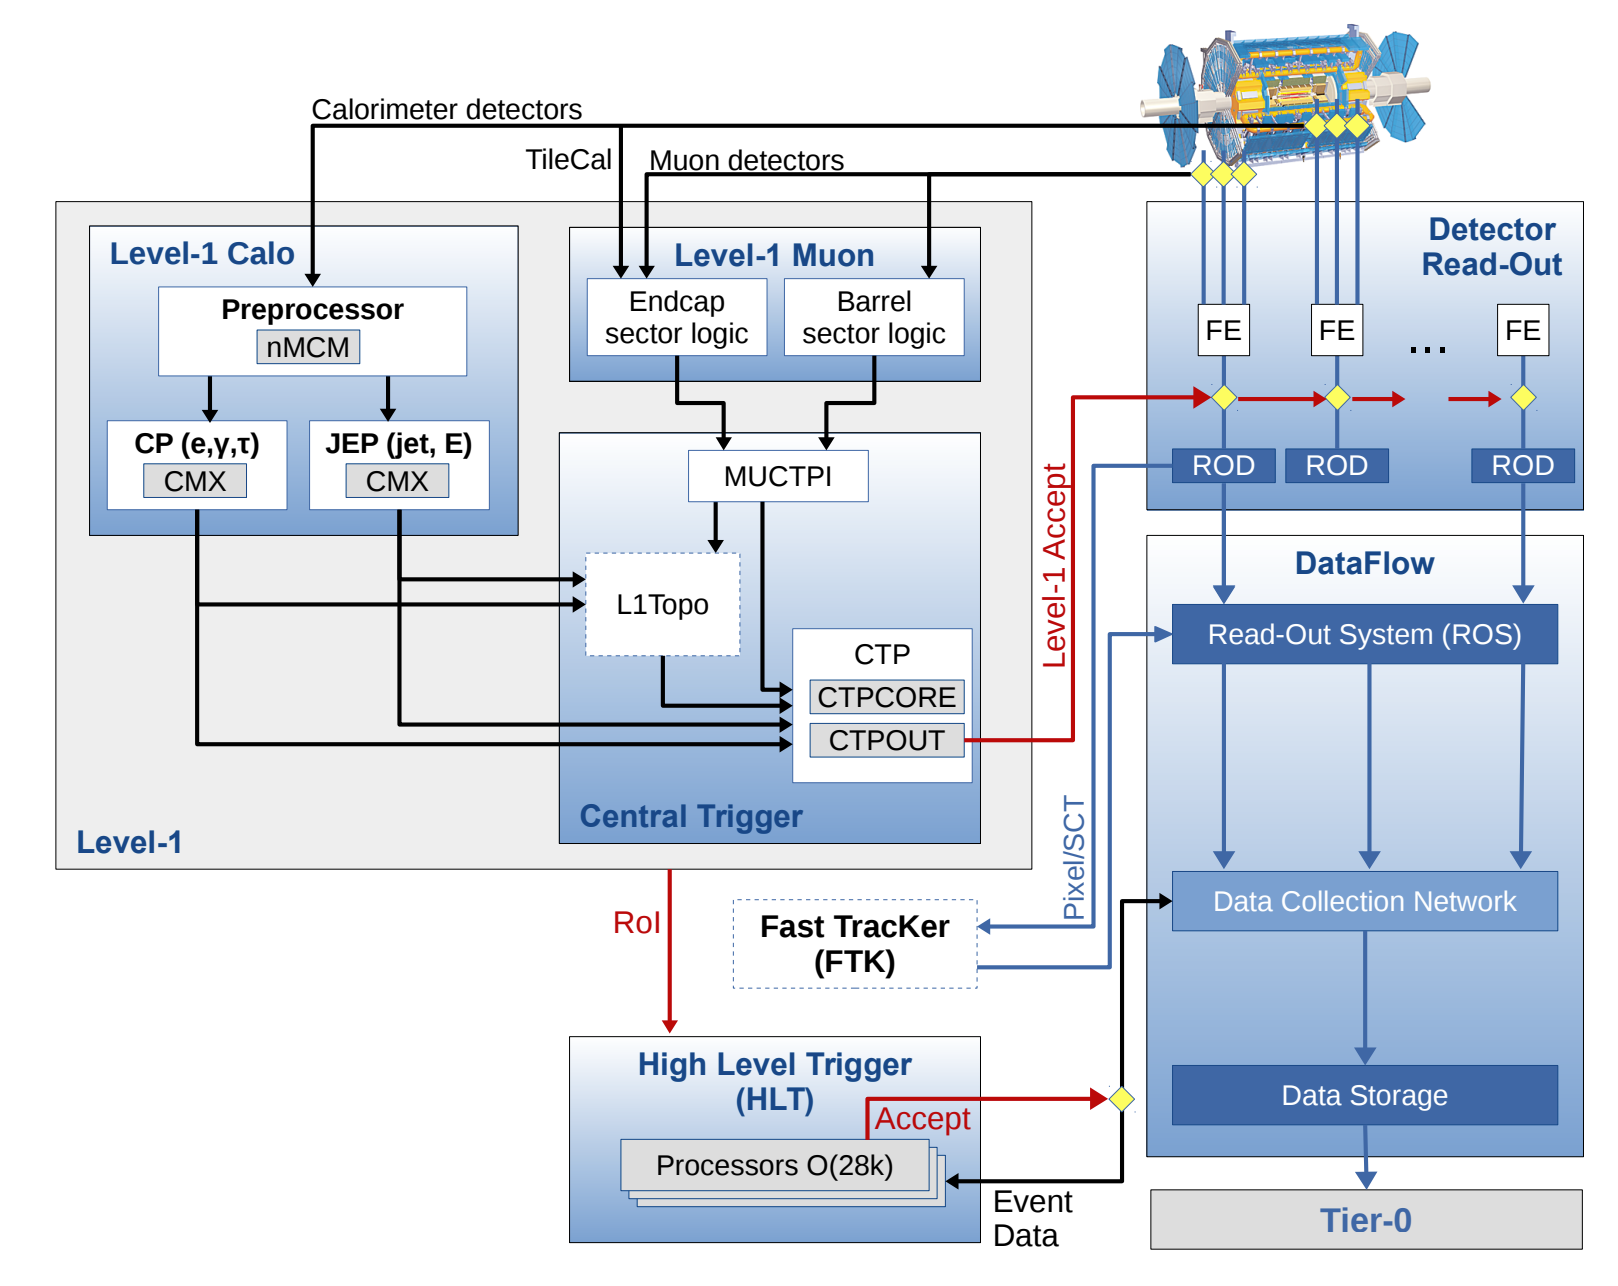
\includegraphics[width=\textwidth]{IDTrig/schematics/TDAQSystem}
\caption{The \ac{ATLAS} \ac{TDAQ} system in Run 2 with emphasis on the components relevant for triggering ~\cite{ATLASTrigger2015}. The \ac{FTK} system was being commissioned during Run 2 was thus not used for the results shown here.}
\label{fig:TDAQ}
\end{figure}  
  
  The ATLAS triggers are configured into different categories. Triggers are generally defined as \textit{trigger chains} which start from a \ac{L1} trigger and specify a sequence of reconstruction and selection steps required for the signature of interest. The naming convention is as follows: 
 $$\mathrm{TriggerLevel\_TypeAndThreshold\_Identification\_Isolation\_L1Thresholds}$$
  Where, "TriggerLevel" refers to either \ac{L1} or \ac{HLT}, "TypeAndThreshold" refers to the type of object that is being triggered (electron, muon, tau, jet, etc.) and its energy threshold.
   If any identification and/or isolation criteria are used, they are appended to the end of the \textit{trigger chain} name
    \ie: \texttt{HLT\_tau25\_medium1\_tracktwo} is a tau trigger at \ac{HLT} level with a 25 GeV threshold, using "medium" identification criteria and have between 1 and 3 tracks in the inner detector ("\textit{tracktwo}"). 
    For \ac{HLT} triggers, any additional \ac{L1} requirements are described in the "L1Thresholds" and appended to the end of the trigger chain.
   
	It is important to note that not all triggers need or are able to run at their full rate, due to the high luminosity achieved at the \ac{LHC} and abundance of trigger objects (\eg\ single jet triggers). 
	In these cases a sub-sample of events passing the trigger requirements are enough. 
	Some triggers have a thus purposefully decreased output rate, known as \textit{prescale}, which can be applied at \ac{L1} and/or at the \ac{HLT}.
	A trigger with a prescale of $N$ would indicate that the trigger accepts 1 out of $N$ events. 
	 
	\section{Level-1 Trigger}
	\label{sec:L1}
	The \ac{L1} trigger decision is performed by the \ac{CTP}, which uses the information gathered by the \ac{L1Calo} and \ac{L1Muon} trigger systems. The \ac{L1Calo} trigger ~\cite{ATLASJINST,ATLASL1CaloTrig} is based on coarse granularity data inputs from the electromagnetic and hadronic calorimeters. 
	It aims to identify high-$E_T$\ objects such as electrons and photons, jets and $\tau$-leptons decaying into hadrons as well as events with large \met\ and large total transverse energy. 
	For electron/photon and $\tau$ triggers isolation can be required. 
	Isolation implies that the energetic particle must have a minimum angular separation from any other significant energy deposit in the same trigger. 
	
	\ac{L1Muon} trigger is based on input signals from the muon trigger chambers: \ac{RPC} in the barrel and \ac{TGC} in the end-caps. The trigger searches for patterns of hits consistent with high-\pt\ muons originating from the interaction region. %The logic provides six independently programmable \pt\ thresholds.
	Muons are not double counted across the different thresholds.
	
	While the \ac{L1} trigger is based only on the multiplicity of trigger objects (or flags indicating which thresholds were passed, for global quantities), information about the geometric location of triggers objects is retained in the muon and calorimeter processors. Once the event is accepted by the \ac{L1} trigger, this information is sent as an \ac{RoI} to the \ac{HLT}.
	Due to the high rate of interactions, the latency, which is the the time taken from the proton-proton collision until the L1 trigger decision, must be kept as short as possible. The design of the trigger requires the \ac{L1} latency to be less than 2.5 $\mu$s. To achieve this aim the \ac{L1} trigger is implemented as a system of purpose-built hardware processes. The \ac{L1} trigger is thus able to reduce the peak data rate from 40 MHz (rate of collision at LHC) down to a more manageable 100 kHz. 
	\section{High-Level Trigger}
	\label{sec:HLT}
	Events that pass the \ac{L1} are buffered by the \ac{ROS} and then processed by the \ac{HLT}. The \ac{HLT} trigger is able to access information not available to the \ac{L1}, such as finer-granularity calorimeter inputs, precision measurements from the \ac{MS} and tracking information from the \ac{ID} pixel and \ac{SCT}. The information provided to the \ac{HLT} is in the form of \ac{RoI}s, which allows for faster reconstruction algorithms as the range of the detector does not need to be processed. 
	The \ac{HLT} triggers reconstruct tracks first using a fast but less accurate reconstruction algorithm, which is able to reject the majority of uninteresting events. Following this first stage a second more precise (but slower) reconstruction algorithm is run using the results of the first stage on the remaining events. Using this software based reconstruction and event acceptance algorithms the \ac{HLT} trigger system is able to reduce the peak input rate from 100 kHz, from the \ac{L1} trigger, down to 1.2 kHz. Events that are accepted by the \ac{HLT} are transfered to a local storage at the experiment site and exported to the \ac{CERN}'s computing centre for offline reconstruction ~\cite{collaboration_2020}. 
		\section{Inner detector Trigger Tracking}
		\label{sec:idtrigtrack}
		As mentioned previously, to reduce precessing time a two-step tracking approach is implemented by the \ac{HLT} triggers: the \textit{fast tracking} and the \textit{precision tracking}.
	The \textit{fast tracking} consists of a trigger specific pattern recognition, while the \textit{precision tracking} relies heavily on offline algorithms, and is seeded with the information from the \textit{fast tracking} step ~\cite{ATLASTrigger2015,ATL-DAQ-PUB-2013-002}.
	
	The tracking of electrons and muons is performed using the standard two-step approach consisting of the \textit{fast tracking} followed by the \textit{precision tracking}. The combination of these two steps is considered to be a single \textit{tracking stage}. The tracking of hadronically decaying taus and $b$-jets is, however, more complex and thus employs a multi-stage approach in order to reduce the volume of the \ac{RoI}, and the processing time that would be required if it were done in a single stage.
	%Electrons and muons tracking utilise a nominal approach, consisting of the two-step tracking mentioned previously, which is considered to be a single \textit{tracking stage}. The hadronic tau and $b$-jet tracking, however, employ a multi-stage approach in order to reduce the detector volume of the \ac{RoI}.
		\subsubsection*{Fast Tracking}
		\begin{figure}[!htb]
	\begin{center}
		\subbottom[]{
			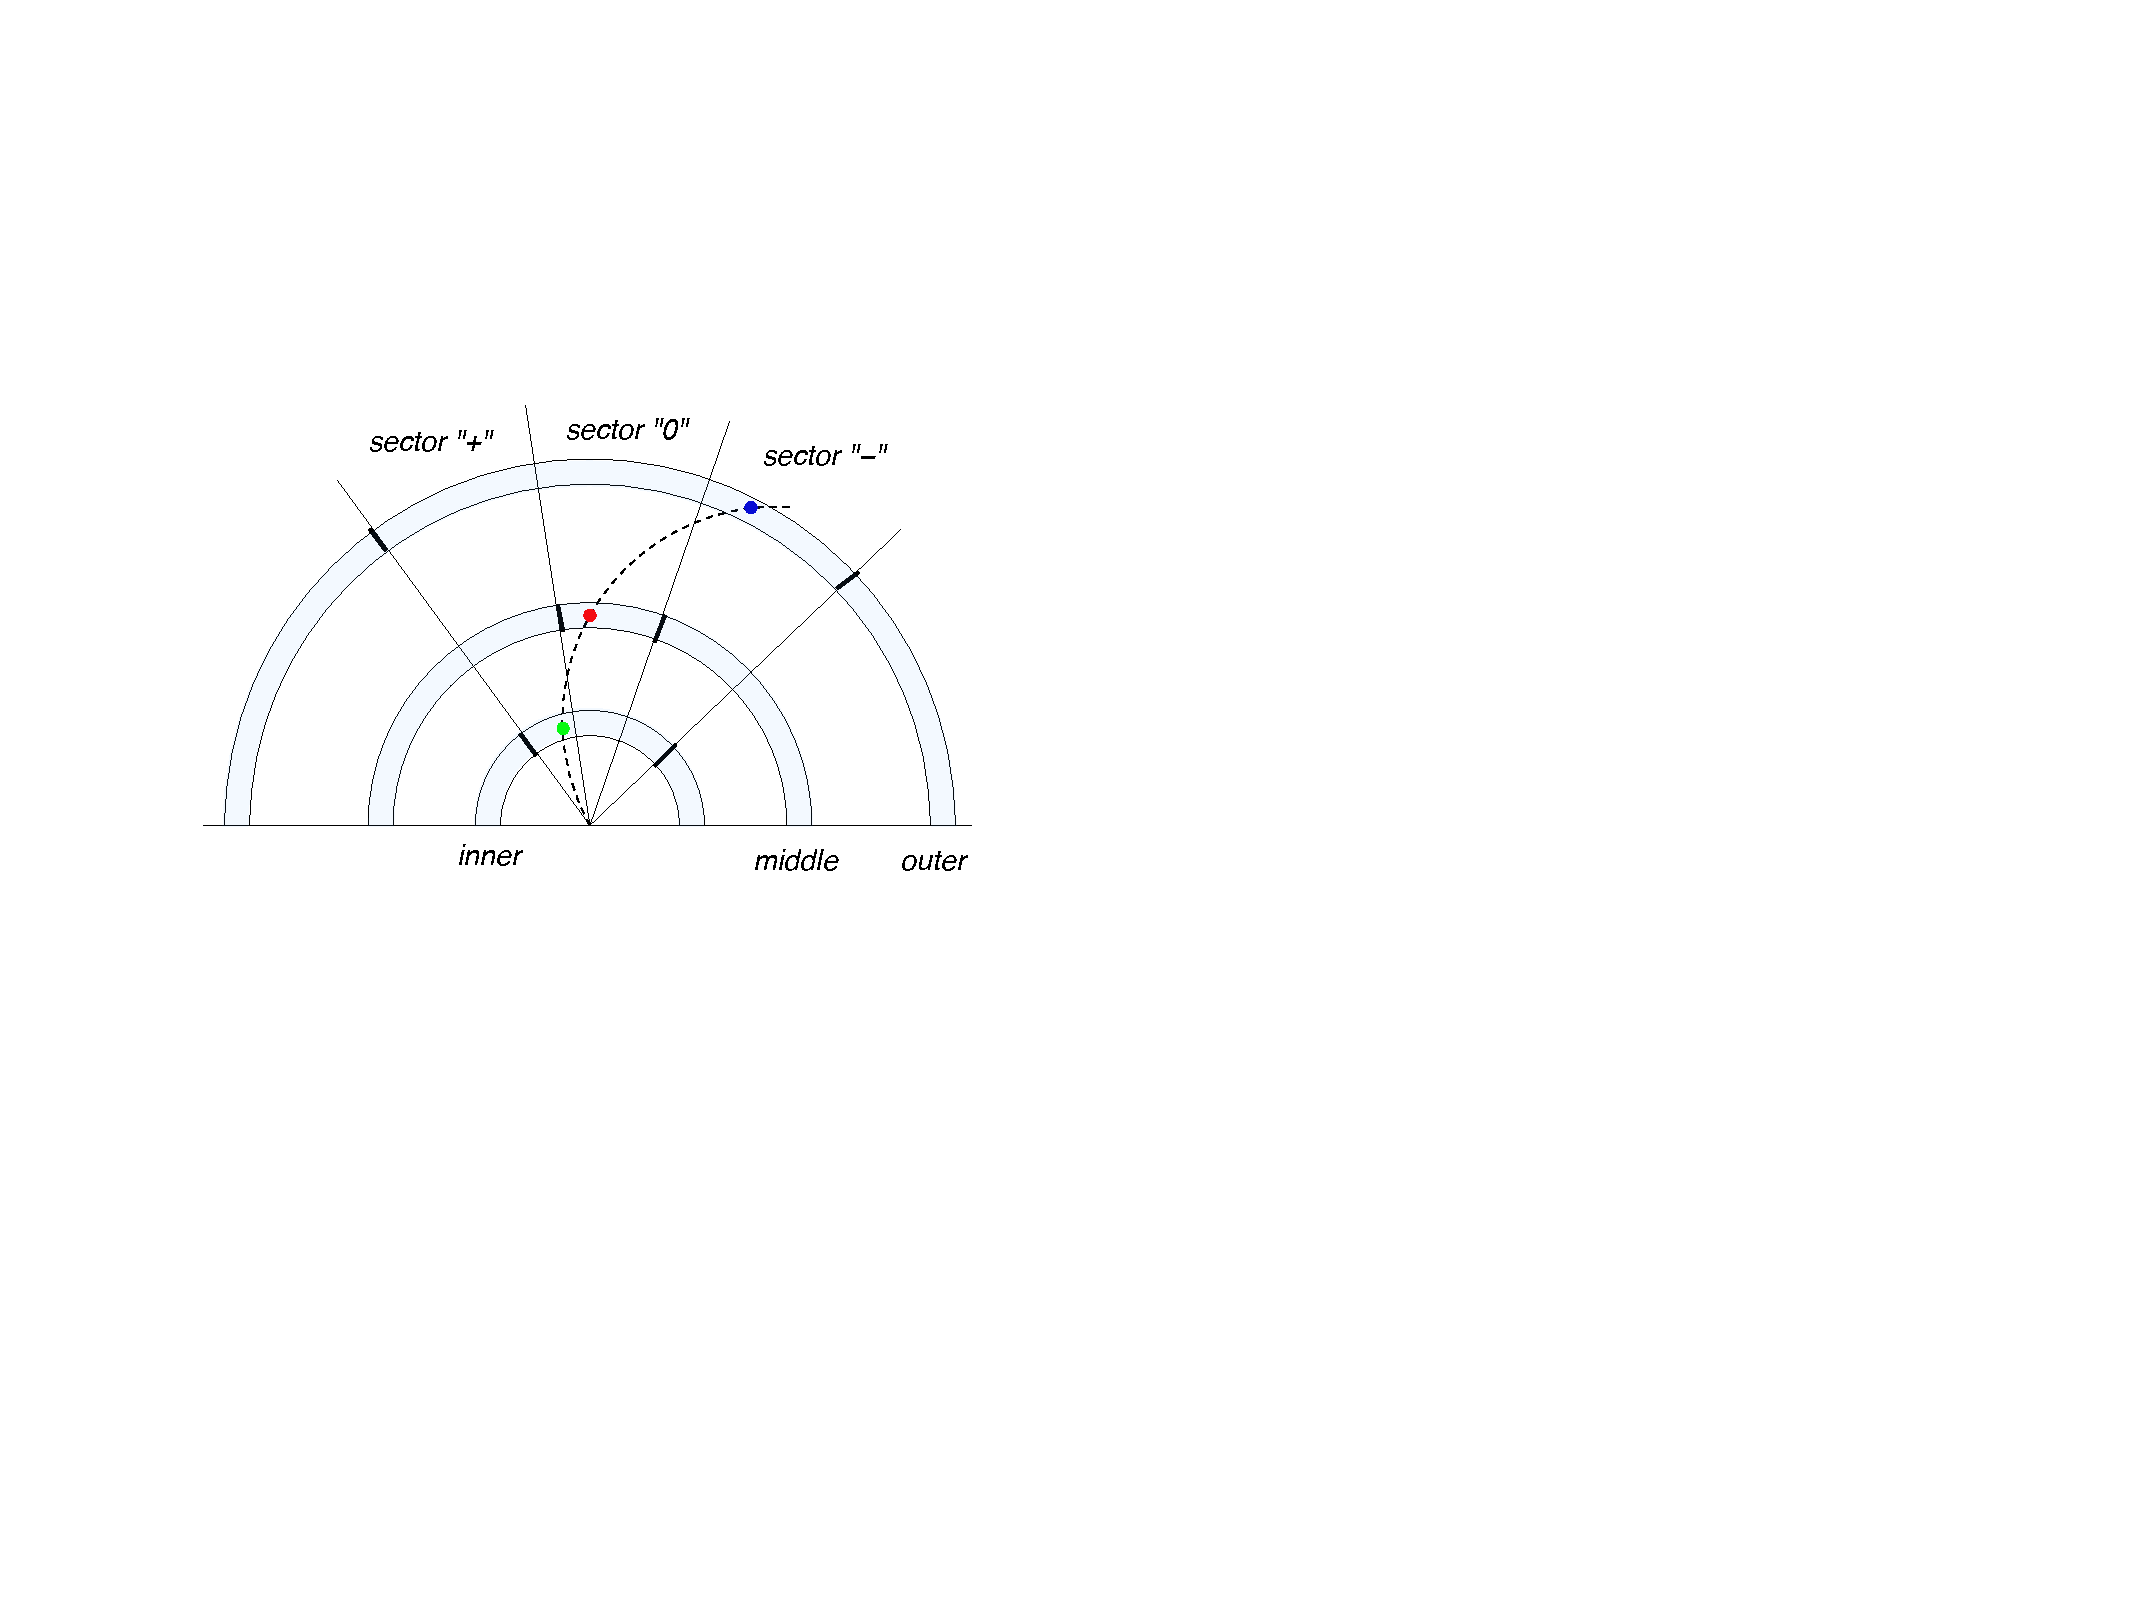
\includegraphics[width=0.45\textwidth]{IDTrig/schematics/seeds-rphi}}\hspace{0.05\textwidth}
		\subbottom[]{
			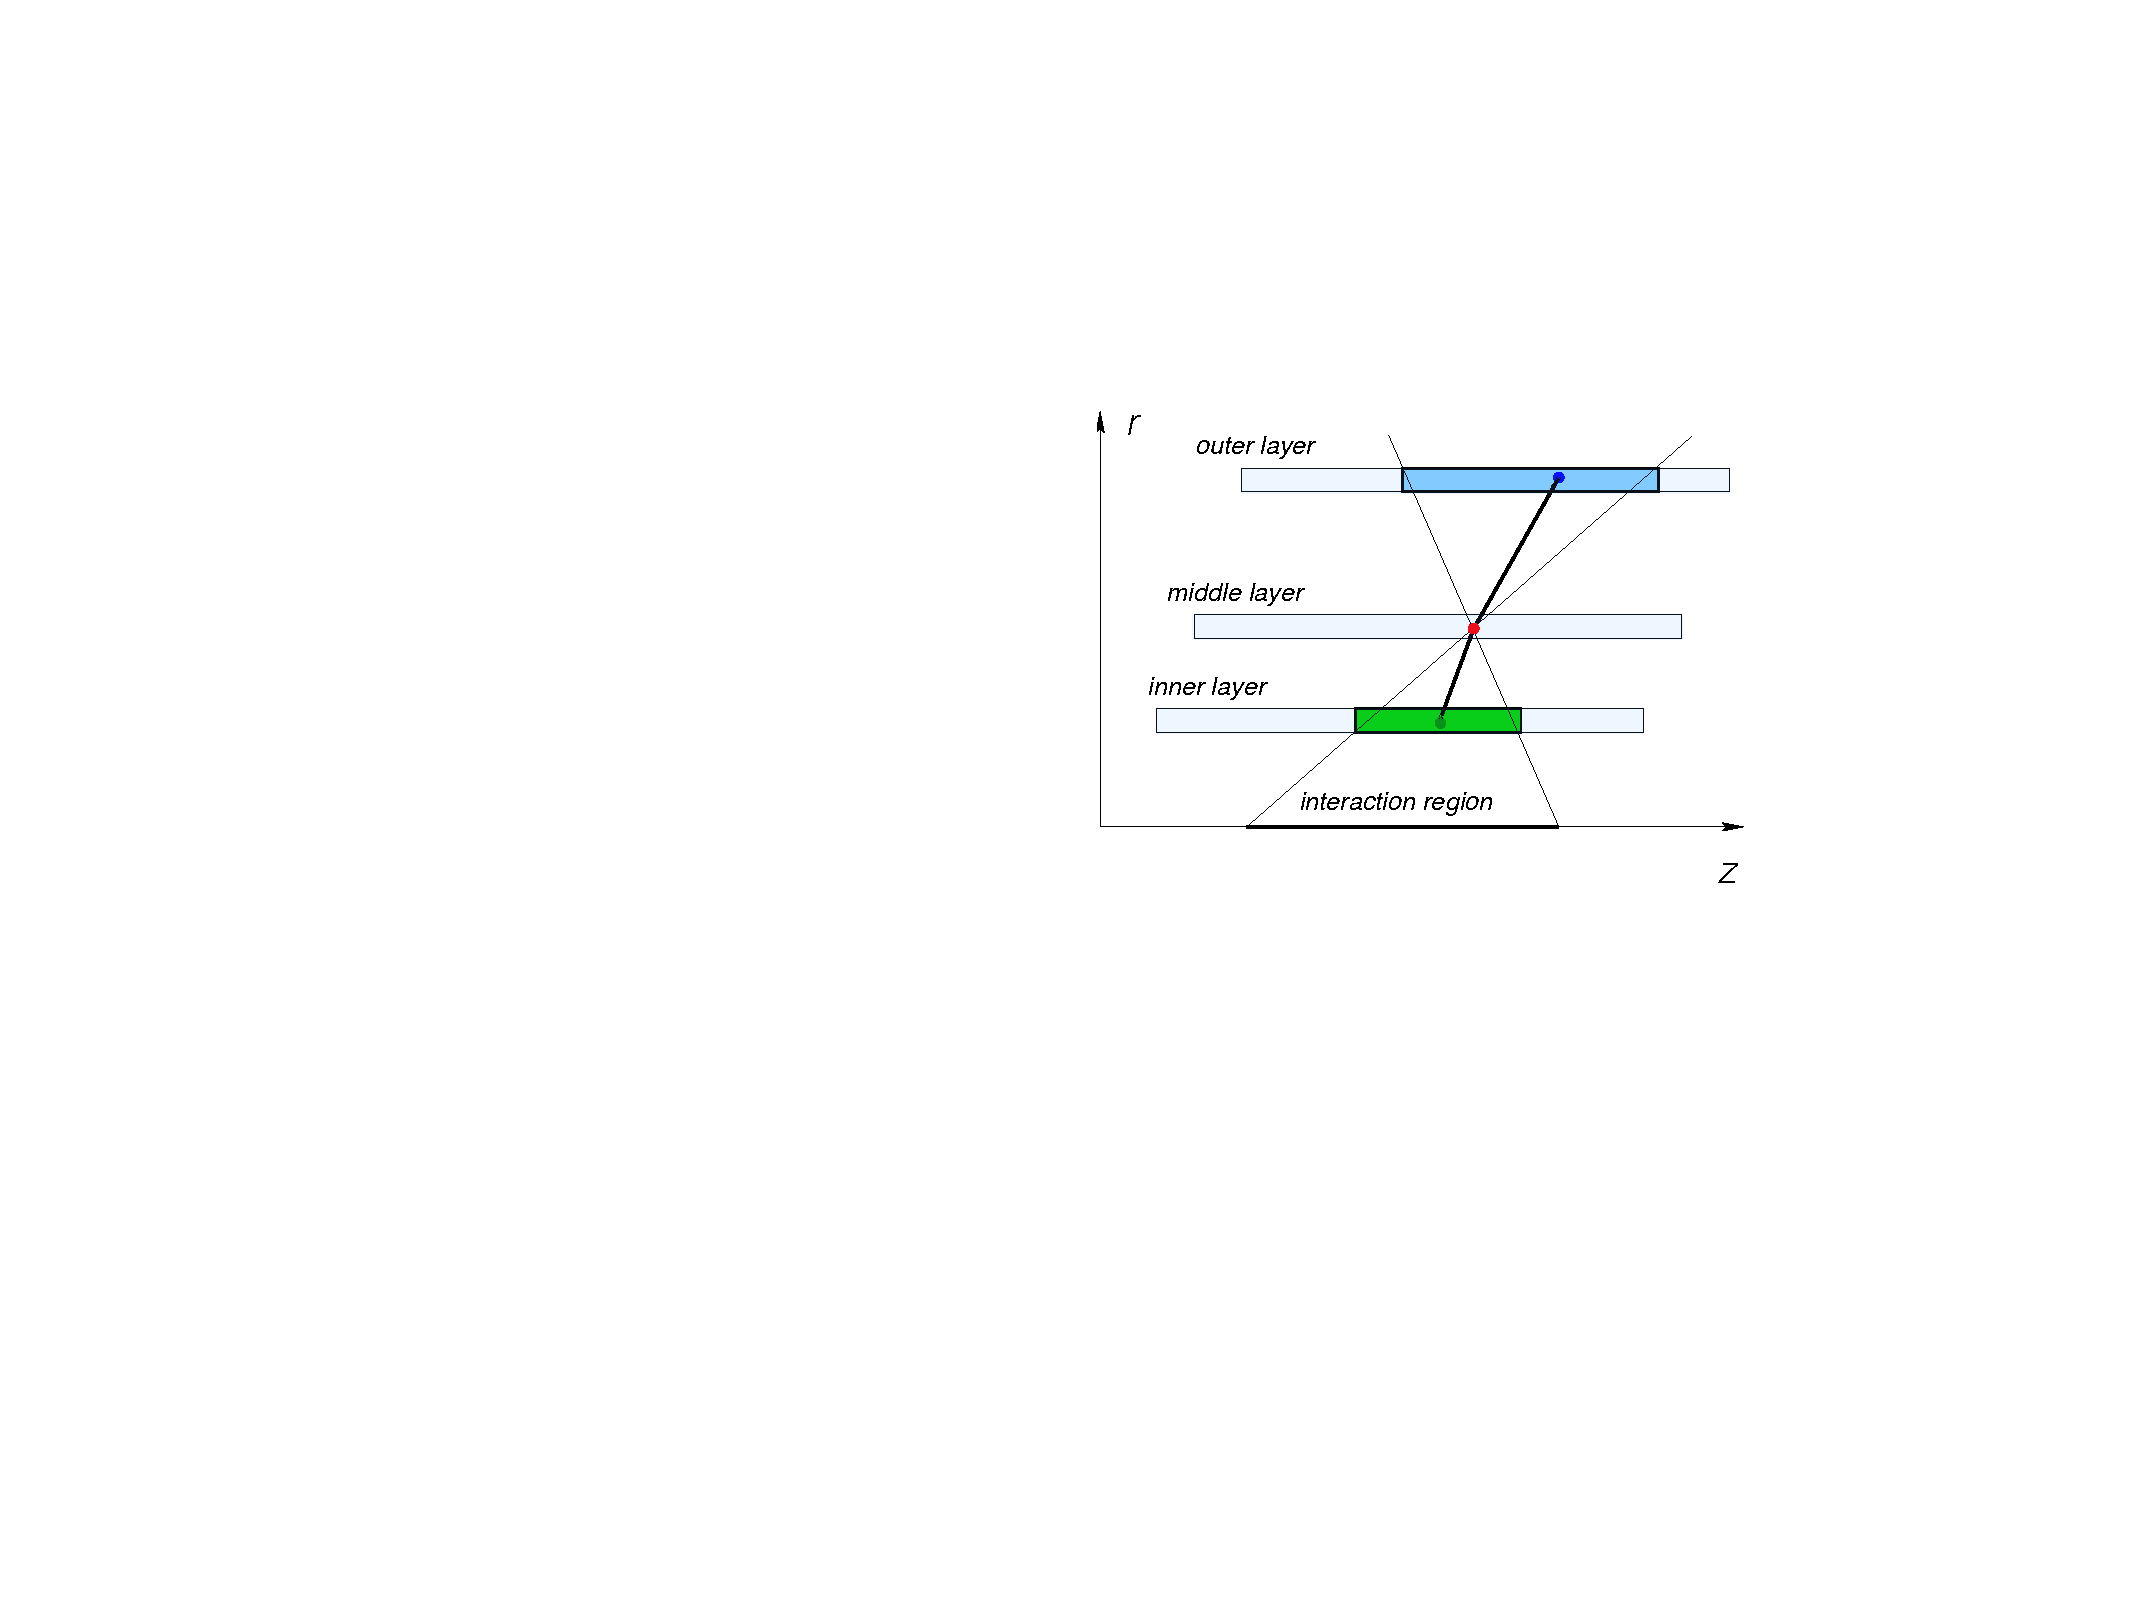
\includegraphics[width=0.45\textwidth]{IDTrig/schematics/seeds-rz}}\hspace{0.05\textwidth}
	\end{center}	
	\caption{Schematics (a) the track seed information in radial bins and azimuthal sections and (b) tracks seed information in the \textit{r-z} plane.}
	\label{fig:schem_FTF}
	\end{figure}	 
	\noindent For the inital stage of track finding in the trigger the \ac{FTF} ~\cite{ATL-DAQ-PUB-2013-002} algorithm was developed to provide track candidates that could be use to seed the precision tracking stage. The \ac{FTF} design therefore prioritises track finding efficiency over purity. The \ac{FTF} pattern recognition is performed by searching for triplets of space-points (\textit{track seeds}) in bins or \textit{r} and sectors of $\phi$, as shown in Figure ~\ref{fig:schem_FTF}. 
	The selection of the triplet begins with the middle space-point, followed by the identification of the \textit{outer} and \textit{inner} space-points at larger and smaller radii respectively. The inner and outer pair of space-points must be compatible with the nominal interaction region along the beam line. 
	This region can be replaced by a restricted \textit{z}-region of the \ac{RoI} along the beam line as also shown by Figure \ref{fig:schem_FTF}, in the case of \ac{RoI} based tracking. 
	The triplet track parameters $\phi_0$, transverse momentum $p_T$, and transverse impact parameter at the point of closest approach to the beam line $d_0$, are estimated using a conformal transformation ~\cite{YEPES1996582}, with the transformation centre placed in the middle space-point and applying cuts on $d_0$ and $p_T$.
	
	Using the track seeds a simple track finding algorithm optimised for speed is utilised to form the initial track candidates. To remove duplicate tracks that share tracks seeds a dedicated algorithm is applied, which retains the tracks of higher quality selected by a fast $\chi^2$ fitter ~\cite{SUTTON2007761}. These preliminary tracks are then passed to the Kalman filter track fitter ~\cite{Kalman1987}. For speed the \ac{TRT} hits are not used in the \ac{FTF}.  Track candidates with too large $d_0$ value (\ie above 10 mm for muons and 4 mm for other signatures) are rejected in order to keep the contributions from fake tracks to a manageable level.
	
		\subsubsection*{Precision Tracking}
		To limit the \ac{CPU} usage the precision tracking stage applies a version of the offline tracking algorithms \cite{Cornelissen_2008,ATLAS-CONF-2010-072}, configured to run online in the trigger ~\cite{CERN-LHCC-97-016,Haywood:331064}, using the \ac{FTF} tracks as inputs. Track candidates are extended into the \ac{TRT} in an attempt to select \ac{TRT} hits at large radii to improve the track momentum resolution. Finally the final \ac{ID} track refit is performed using a more precise $\chi^2$ fitter algorithm ~\cite{chi2fit}.
		
		The rate of processing for the precision tracking is generally significantly lower than for the fast tracking.
		This allows for a more detailed handling of the detector conditions and better compensation for detector effects (\ie\ inactive sensors or calibration corrections). This results in the precision tracks being much closer in performance to the offline tracks than to the fast tracks. 
		Since the precision tracking uses the tracks and clusters identified by the fast tracking, by definition, the precision tracking efficiency cannot exceed that of the fast tracking.
		
		The overall purpose of the precision tracking is to perform a higher quality fit to improve the purity and quality of the trigger tracks identified by the first stage \ac{FTF}.
			
			\subsubsection*{Vertex Reconstruction}
		Two vertex reconstruction algorithms are used online: a histogramming based algorithm, and the offline vertex algorithm ~\cite{ferrari2007tracking,ATLAS-CONF-2012-042}. 
		Typically, trigger signatures use the offline vertex algorithm, with the exception of the $b$-jet trigger which uses both algorithms to maximise the vertex finding efficiency. 
		The simple histogramming algorithm works by histogramming the $z_0$ position for the point of closes approach to the beam line of each track and then calculates the vertex $z$ position. 
		This is done by using the mean of the bin centres weighted by the number of tracks in each bin for the group of adjacent bins within the 1 mm sliding window which contains the largest number of tracks. 
		All tracks passing some basic quality selection are used and are weighted equally. 
		The second algorithm is based on the offline vertex finder algorithm ~\cite{ATLAS-CONF-2012-042} with modifications applied for online running. 
		Both algorithms only run on tracks that have been reconstructed in the relevant \ac{RoI} of the track finding.  
		
		\subsubsection*{Multistage Tracking} 
	As mentioned previously, the fast and precision tracking algorithms run in distinct stages, but are considered to be part of a single \textit{tracking stage}, because there is only a single pass of the tracking over any specific \ac{RoI}. 
	Performing multiple passes of aspects of the tracking is referred as \textit{multistage} tracking. Multistage tracking can run multiple aspects of the tracking in different steps, updating the constructed \ac{RoI} at each step.
	
	The generic structure of the multistage tracking is illustrated in Figure ~\ref{fig:multi_stage} where in a region of the detector the first stage fast tracking is performed over an \ac{RoI} to identify the event vertex.
	 Given the results of the first stage the dimensions of the \ac{RoI} are changed into a different \ac{RoI}. 
	  The second stage executes the fast tracking again, followed by the precision tracking for the tracks found in this second fast tracking stage, run in this new \ac{RoI}. This process is trigger specific and will be discussed in more details for the relevant object below.
	%\begin{wrapfigure}{R}{.45\textwidth}
	\begin{figure}[!hbt]
	\centering
	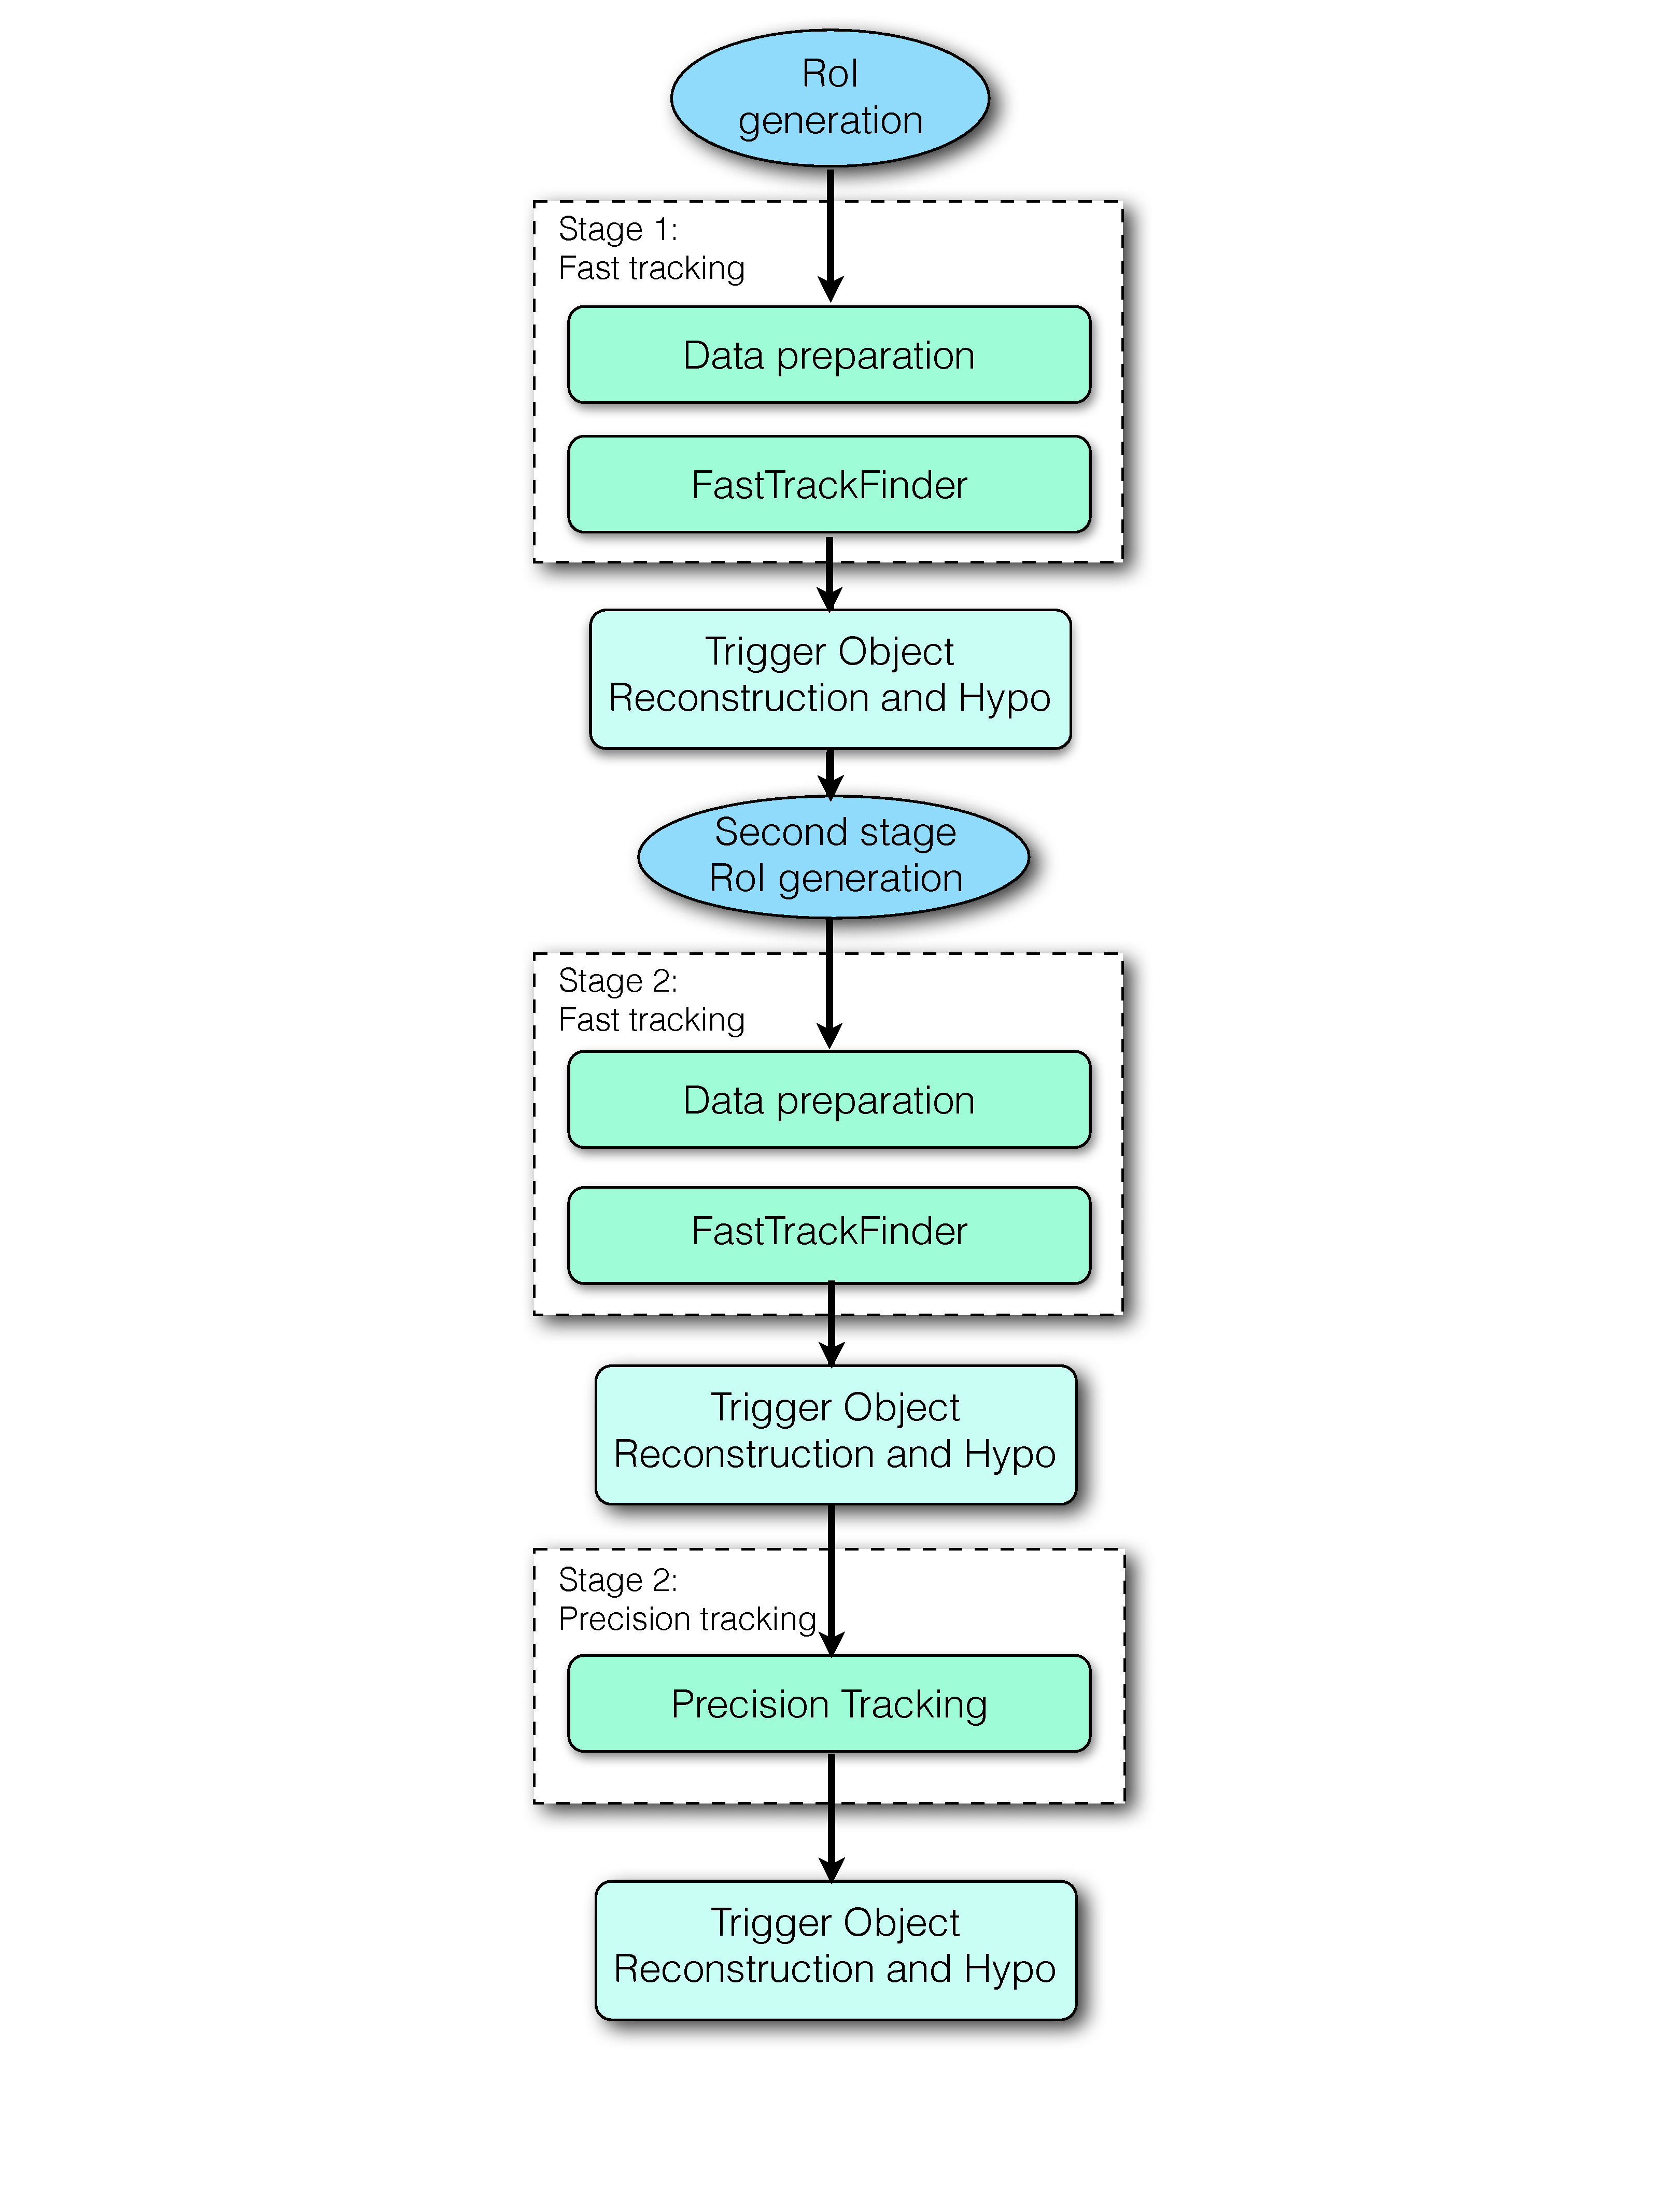
\includegraphics[height=0.55\textheight]{IDTrig/schematics/multi-stage}
	\caption{Schematics illustrating multistage tracking. And initial first stage is fast tracking performed on an \ac{RoI}, followed second fast and precision tracking stages run over a second stage \ac{RoI}.}
	\label{fig:multi_stage}
	\end{figure} 
%\end{wrapfigure}

	Hadronic tau triggers require a larger \ac{RoI} than for instance, electrons, to allow for the opening angle of the tracks from the three prong decay. To limit the tracking \ac{CPU} usage in this wider \ac{RoI} a mutlistage approach us used, as illustrated by Figure ~\ref{fig:roi_tau}. 
	In the first stage the fast tracking is run to identify the position of tau event vertex and leading track along the beam line in a narrow \ac{RoI} with a full width of 0.2 in both $\eta$ and $\phi$, but fully extended along the beam line in the range of $|z|<$ 225 mm, represented by the purple area in the diagram. The \ac{RoI} is then changed to a wider version with full width 0.8 in both $\eta$ and $\phi$, centred on the $z$ position of the leading track identified by the first stage (as shown by the blue area on the diagram) and limited to $|\Delta z|<$ 10 mm with respect to the leading track. The fast tracking is performed in this wider \ac{RoI}, followed by the precision tracking for the tracks found in this second fast tracking stage. Even though the multistage tracking runs the tracking algorithms repeatedly for the two stages, the combined tracking volume of the first and second stage is still significantly smaller than for the \ac{RoI} in the single-stage tracking scheme. 
	\begin{figure}[!hbt]
	\centering
	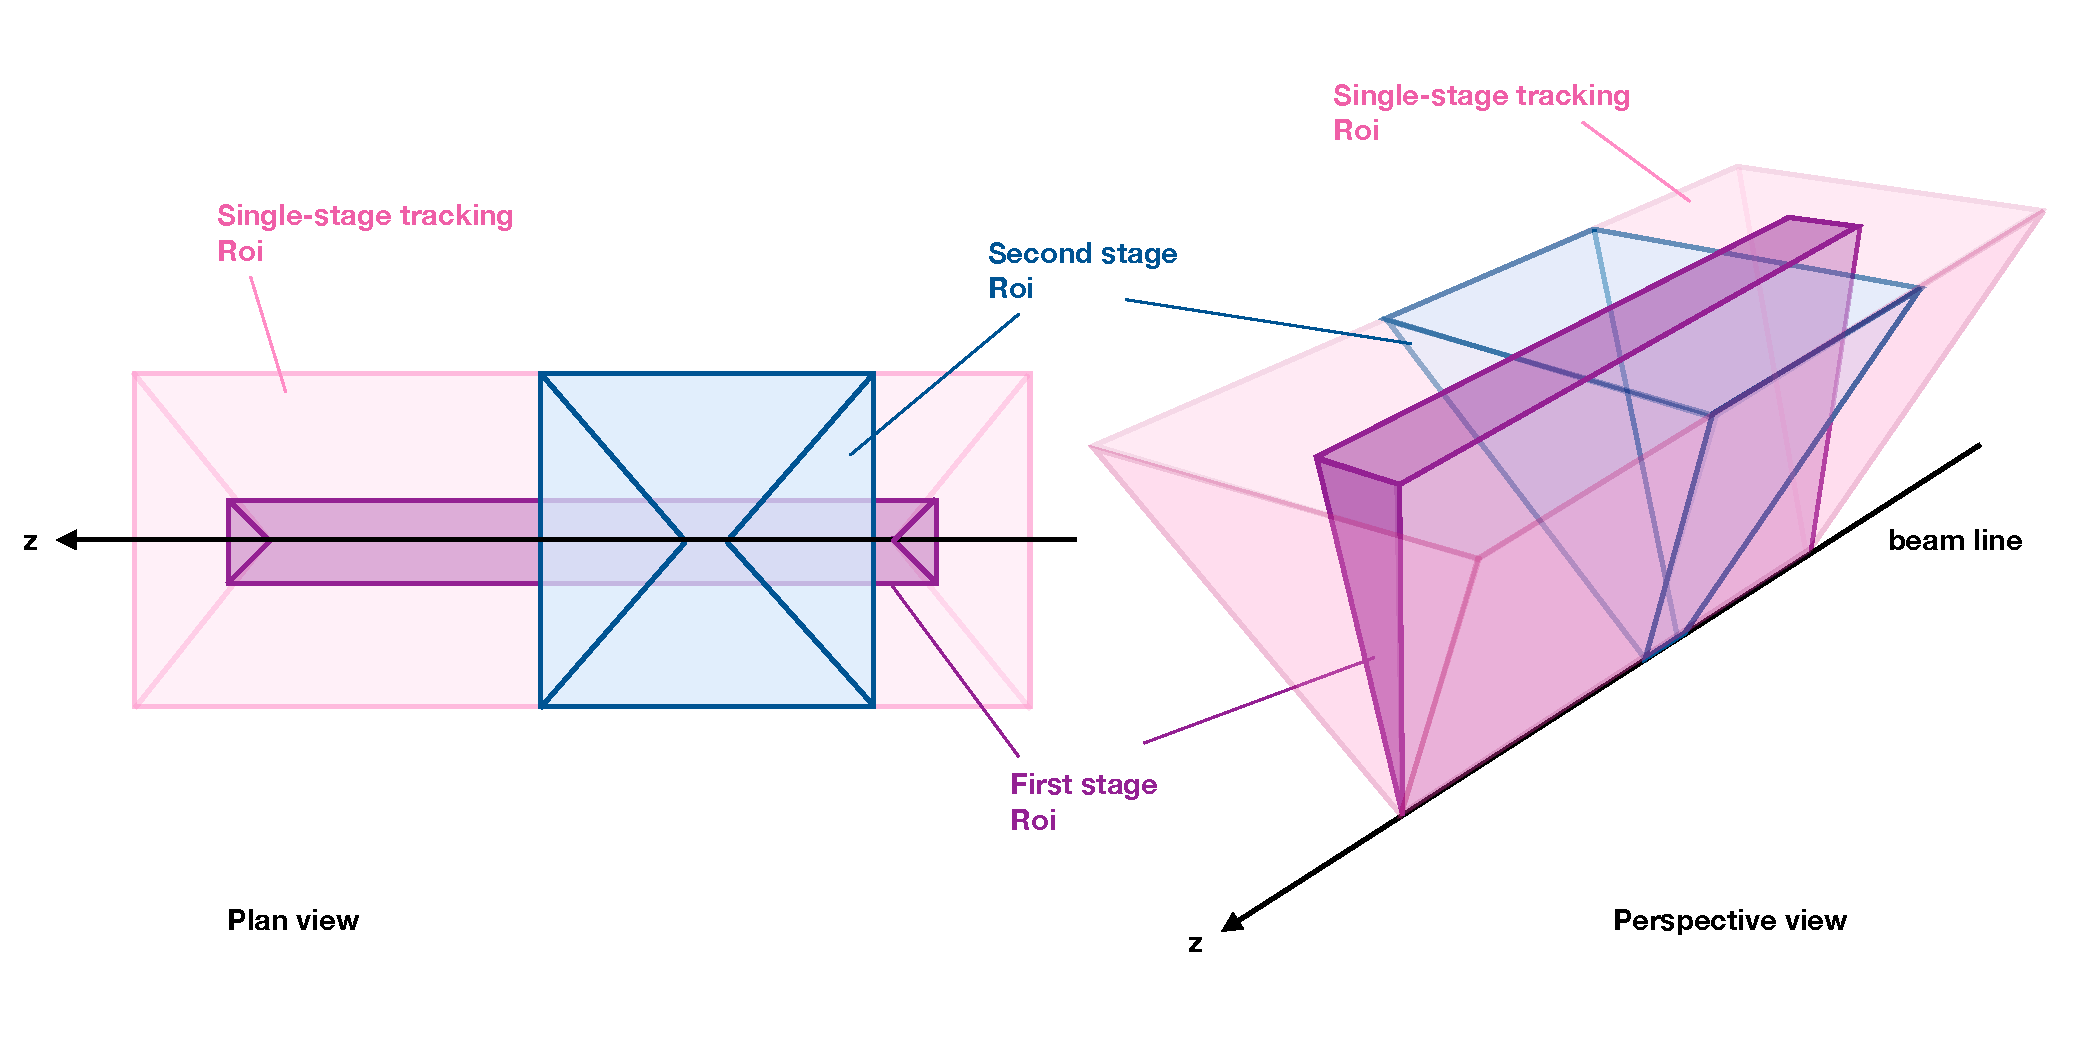
\includegraphics[width=\textwidth]{IDTrig/schematics/roi-tau}
	\caption{Schematics illustrating the \ac{RoI}s from the single-stage and two-stage tau lepton trigger tracking shown in plan view, ($x-z$ plane) along the transverse direction, and in perspective view, with the $z$-axis along the beam line. The combined volume of the first and second stages of the two-stage tracking approach (blue and purple areas respectively) is noticeably smaller than the \ac{RoI} in the single-stage (pink area) tracking scheme.}
	\label{fig:roi_tau}
	\end{figure} 

The multistage approach reduces the mean processing time for the hadronic tau trigger fast tracking from 66.2 $\pm$ 0.34 ms for the single-stage, down to 23.1 $\pm$ 0.11 ms and 21.4 $\pm$ 0.09 ms for the first and second stages of the multistage approach, respectively. For the precision tracking the mean processing time was reduced from 12.0 $\pm$ 0.07 ms for the single-stage down to 4.8 $\pm$ 0.04 ms using the multistage ~\cite{Sutton:2695048}.

	A similar multistage tracking strategy is adopted for the $b$-jet trigger. In the first stage the vertex tracking is used to identify the likely event vertex $z$ position for use in the second stage for jets identified by the jet trigger with transverse energy $E_T\,>\,30$ GeV. 
	For the second stage, separate \ac{RoI}s about each jet, specialised more tightly at the beam line about the $z$ vertex position identified in the first stage, are used. 
	The tracks are then reconstructed with the fast tracking algorithm in a narrow region with full width of 0.1 in $\eta$ and $\phi$ around the jet axis of each jet, but with $|z|\,<$ 225 mm along the beam line.
	 To prevent multiple processing of overlapping regions of the detector, before running the fast tracking, the \ac{RoI}s about each jet axis are aggregated into a \textit{super \ac{RoI}}, as shown by Figure ~\ref{fig:superroi}.
	  This super  \ac{RoI} is used to determine which detector elements should be read out by the data preparation stage.
	
	Following this stage the tracks identified in the super \ac{RoI} are used for the primary vertex reconstruction ~\cite{Meloni_2016}. This vertex is used to define wider \ac{RoI}s with $|\Delta\eta|$ and $|\Delta\phi|$ less then 0.4 each, with respect to the jets axis, but with $|\Delta z|\,<$ 10 mm relative to the primary vertex $z$ position.
	These \ac{RoI}s are used for the second-stage reconstruction which runs the fast tracking in a wider $\eta$ and $\phi$ regions about the jets. The precision tracking, primary vertexing and $b$-tagging algorithms are all subsequently run. As in the case of the tau multistage tracking, the use of this multistage process reduces significantly the mean processing time. 
	\begin{figure}[!hbt]
	\centering
	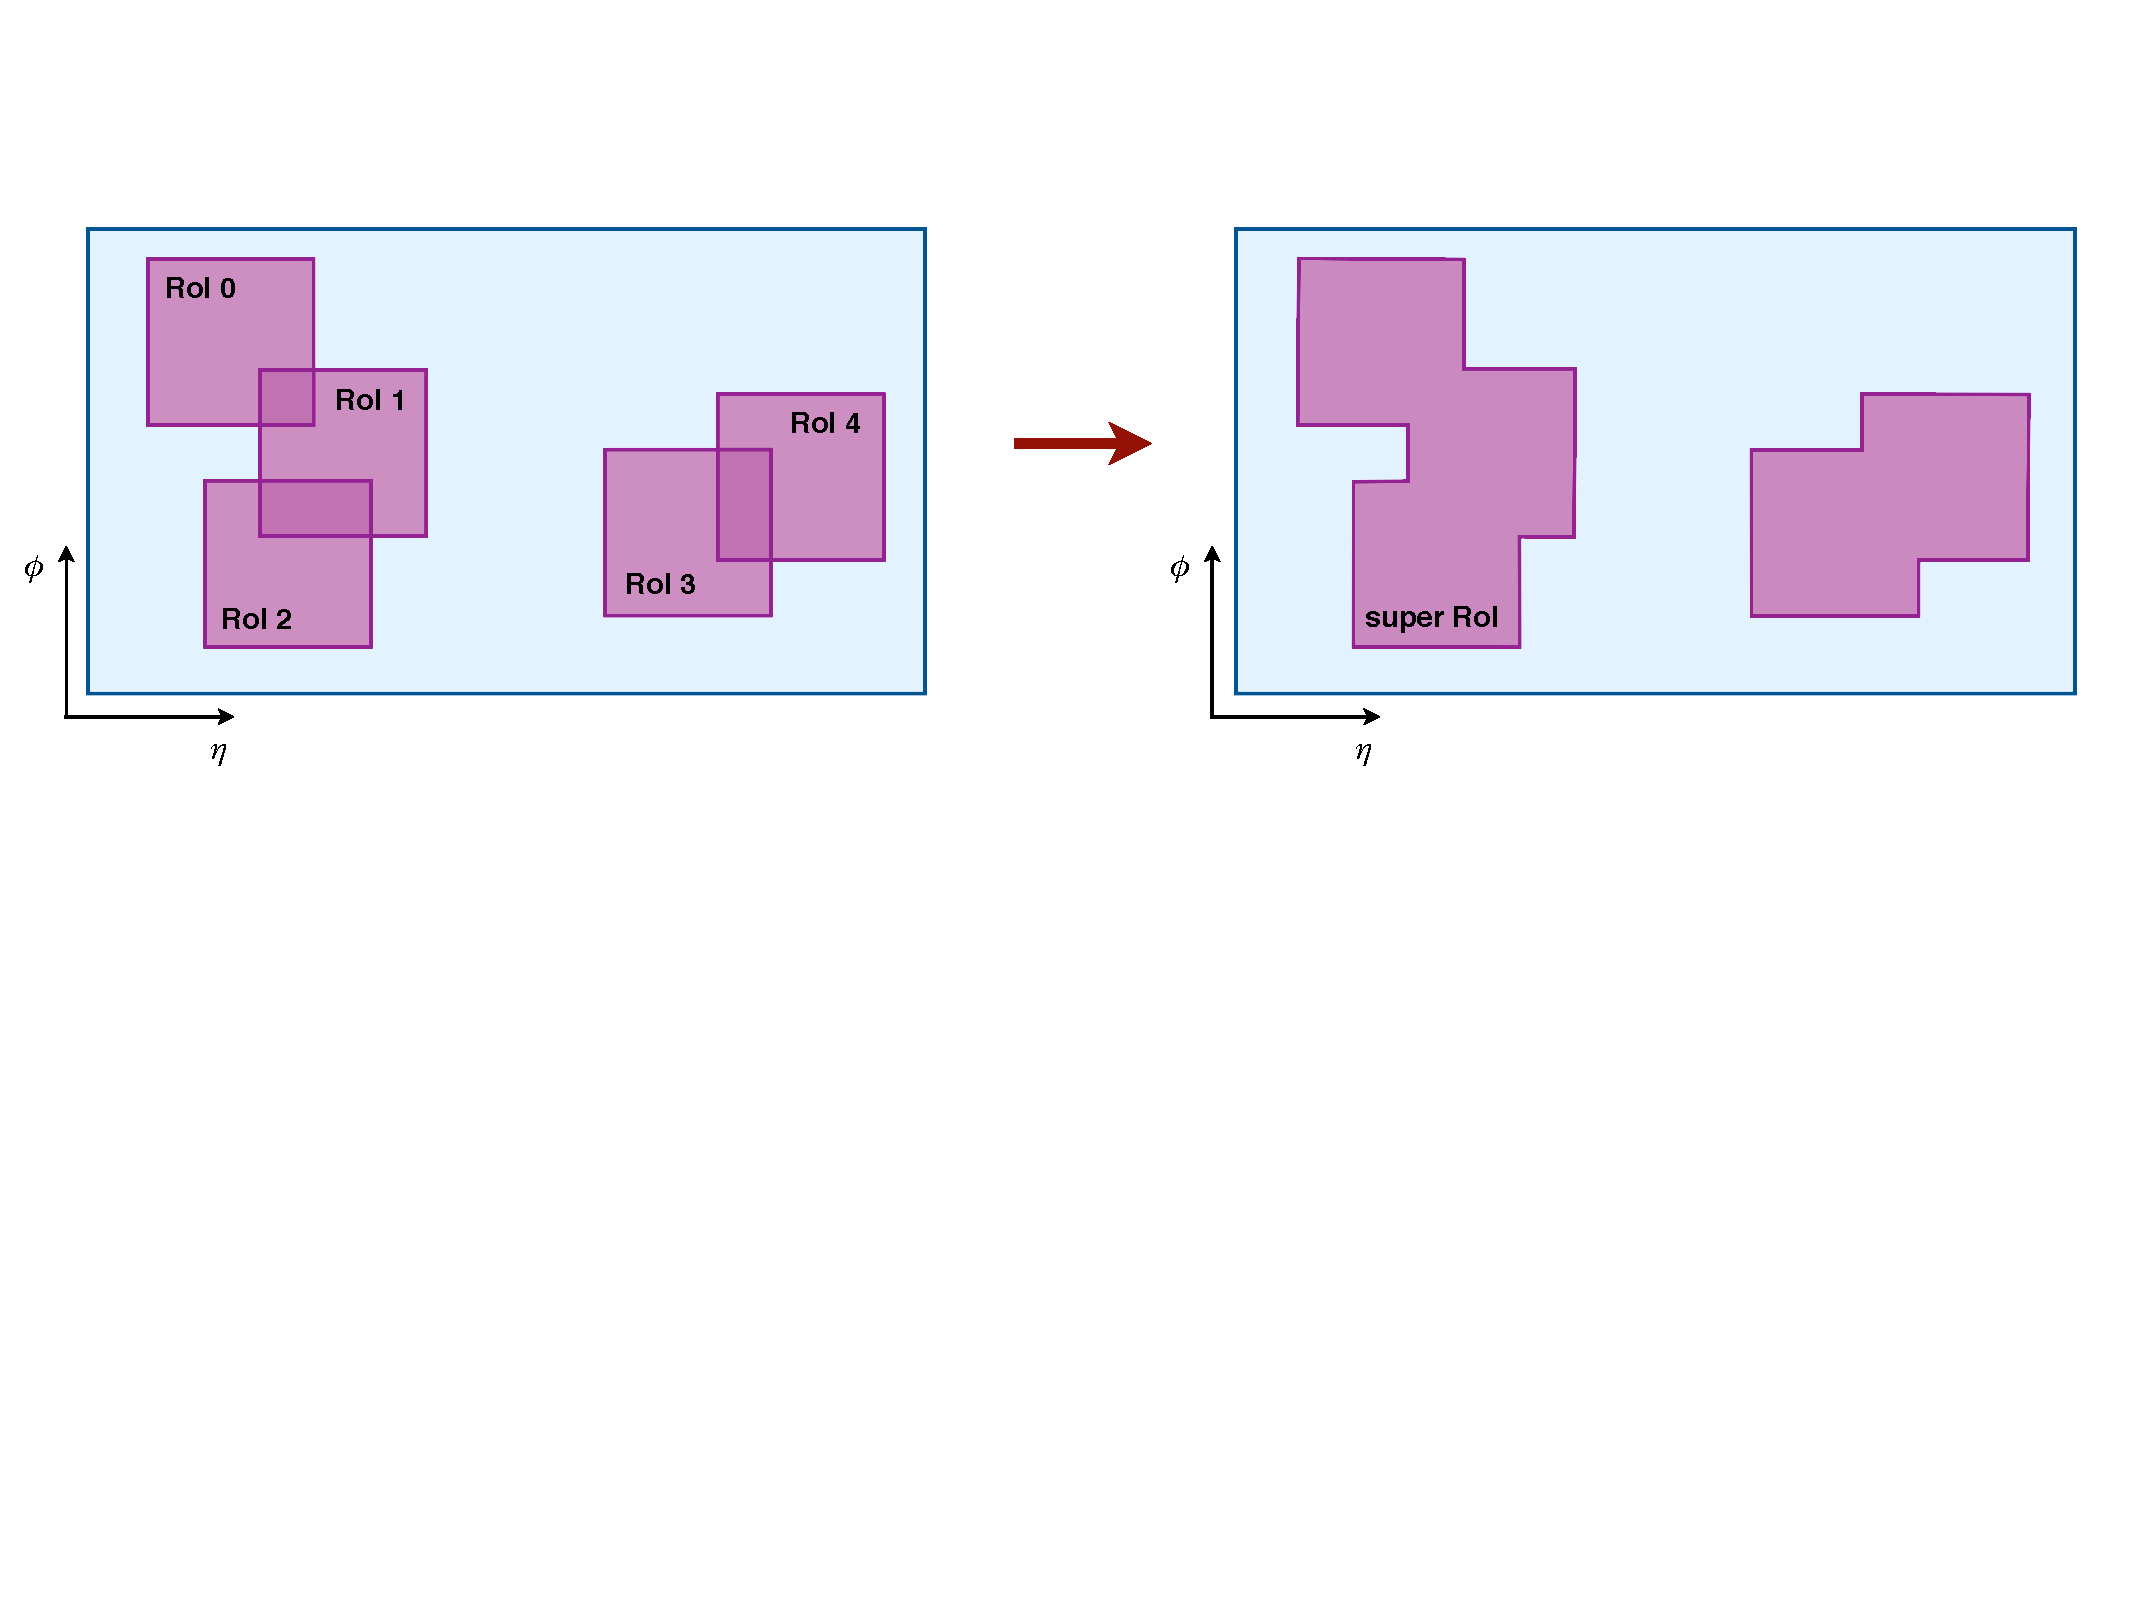
\includegraphics[width=\textwidth]{IDTrig/schematics/superroi}
	\caption{A schematic illustrating the creation of the super \ac{RoI} from all the trigger jets reconstructed with an $E_T\,>$ 30 GeV.}
	\label{fig:superroi}
\end{figure} 

	
	\section{ID tracking Performance}
	\label{sec:idtrigperf}
	The performance of muon and electron triggers is presented for the full available luminosity for the 2016-2018 data collection period, collected at the \ac{ATLAS} experiment using 13 TeV $pp$ collision events. This was possible since the processing for these triggers did not change significantly throughout data taking. For the tau and $b$-jet signatures, which ran multistage tracking, significant changes were made to the reconstruction of either the first or second stages of the multistage process over the data collection period. These changes include the modification to the second stage seed finding. Therefore only results for 2018 are  presented in full details for these signatures. 
	
	To remain as unbiased as possible, specific monitoring triggers that do not require a track to be present for the event to be accepted are used for the estimation of efficiency of the tracking. 
	The efficiency, residuals and resolutions presented below are calculated with respect to the tracks found by the offline reconstruction software ~\cite{Cornelissen_2008}. The efficiency is therefore defined as the fraction of offline reference tracks that are matched to a trigger track
%mathscr
	\begin{equation}
	\pazocal{F}\,=\,\frac{\mathrm{N_{trigger}}}{\mathrm{N_{offline}}},
	\end{equation}
	where $\mathrm{N_{trigger}}$ is the number of tracks matched to a trigger and $\mathrm{N_{offline}}$ is the number of tracks reconstructed by the offline reconstruction software.
	For any given offline track, the reconstructed track that matches the closest to a loose preselection cone of size $\Delta R\,=\,\sqrt{(\Delta\eta)^2+(\Delta\phi)^2}\,=\,0.05$ to the offline track, is chosen as a match. 
	%The reconstructed tracks are considered matched to an offline track if they are 
		\subsection*{Muon trigger}
		Figure ~\ref{fig:muon_idtrig_perf} shows the tracking efficiency for medium quality ~\cite{cite-key} offline muon candidates, using a range of HLT triggers ~\cite{ATLAS-CONF-2012-099} to cover the whole transverse momentum reconstruction spectrum down to 4 \gev, for the fast and precision tracking.  
		Two representative thresholds are used for the offline muon selection: $p_T\,>$ 4 \gev\ corresponding to the lowest trigger threshold, and $p_T\,>$ 20 \gev for the higher trigger thresholds. 
		The efficiency shown for both the fast and precision tracking is significantly better than 99\% and flat as a function of pile-up interaction multiplicity. The small apparent loss in precision tracking for higher \pt\ tracks is primarily caused by the offline reconstruction. Poorly reconstructed candidates of lower \pt\ are occasionally mis-reconstructed at higher momentum by the offline reconstruction, thus creating a larger expected contribution in the reference sample in the high \pt\ region. Therefore poorly offline reconstructed low \pt\ tracks cause the apparent loss in efficiency at higher \pt. It is therefore not an inefficiency that derived from the online \ac{ID} triggers.
		\begin{figure}[!htb]
	\begin{center}
		\subbottom[]{
			\includegraphics[width=0.45\textwidth]{IDTrig/performance/muon/HLT_pT_eff}}\hspace{0.05\textwidth}
		\subbottom[]{
			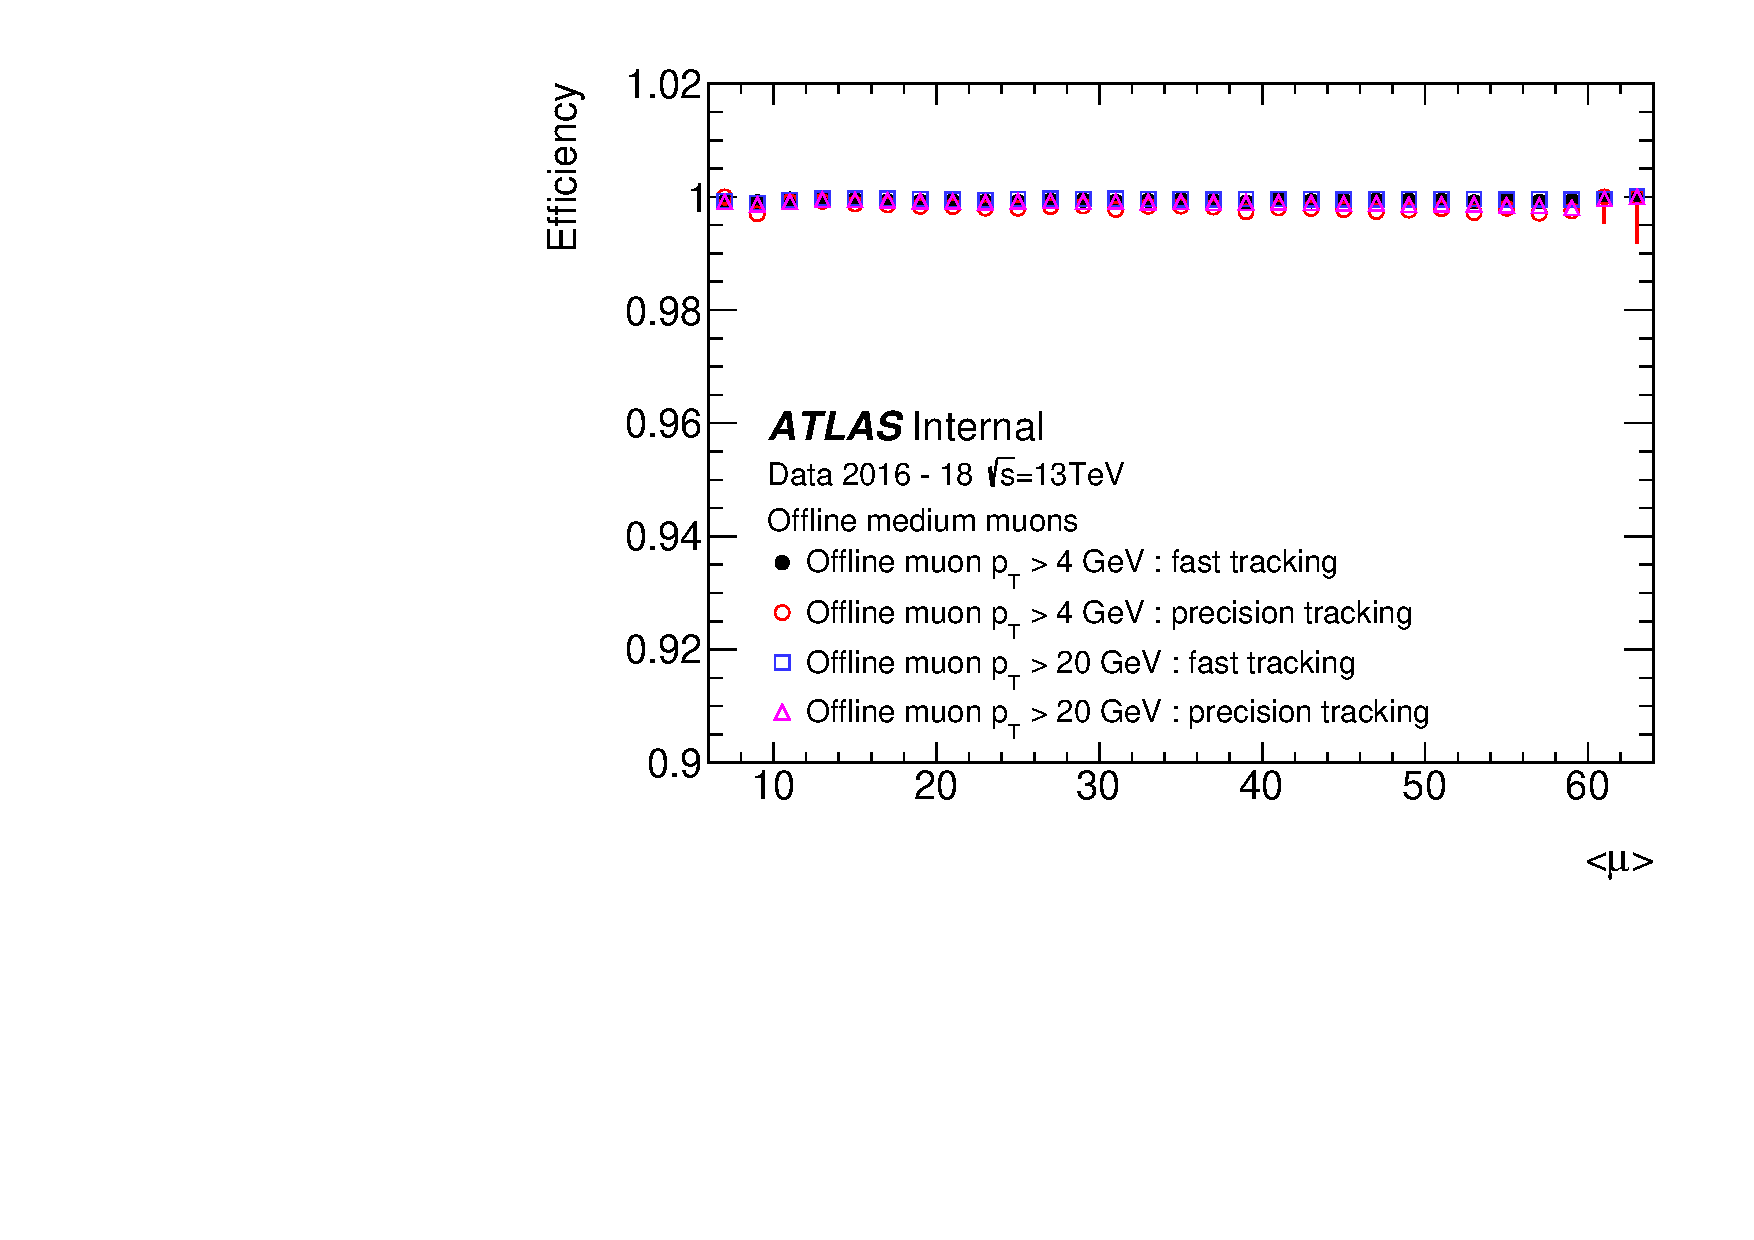
\includegraphics[width=0.45\textwidth]{IDTrig/performance/muon/HLT_eff_vs_muRebin2}}\hspace{0.05\textwidth}
	\end{center}	
	\caption{\ac{ID} trigger efficiency as a function of (a) the offline reconstructed muon \pt, (b) the mean pile-up interaction $<\mu>$ for muons selected by 4 GeV and 20 GeV muon support triggers with respect to medium offline muon candidates with \pt\ $>$ 4 GeV or \pt\ $>$ 20 GeV.}
	\label{fig:muon_idtrig_perf}
	\end{figure}	 
	
	The resolutions for the trigger tracks in $\eta$ and $d_0$ with respect to the offline muon candidate pseudorapidity and \pt\ are shown in Figure ~\ref{fig:muon_idtrig_res}. The fast and precision tracking $d_0$ resolutions are found to be better than 25 $\mu$m and 20 $\mu$m respectively, for muons candidates with offline \pt\ $>$ 4 GeV. The difference in resolution between the two algorithms is due to the fact that the precision tracking performs a higher quality fit using the space points identified by the fast tracking, which improves the purity and quality of the trigger tracks. The degrade of resolution observed at larger pseudorapidities is predominantly due to the increased amount of material through which tracks must travel. The position of the endcap silicon detectors (perpendicular to the beam line) partially ameliorate this, the effect of which can be seen for presudorapidities larger than 1.2 which is the approximate boundary between the barrel and endcap silicon detectors.
		\begin{figure}[!htb]
	\begin{center}
		\subbottom[]{
			\includegraphics[width=0.45\textwidth]{IDTrig/performance/muon/HLT_rd0_vs_pt_sigma}}\hspace{0.05\textwidth}
			\subbottom[]{
			\includegraphics[width=0.45\textwidth]{IDTrig/performance/muon/HLT_reta_vs_eta_sigma}}\hspace{0.05\textwidth}
	\end{center}	
	\caption{\ac{ID} trigger track resolution for (a) transverse impact parameter with respect to the beam line ($d_0$) and (b) pseudorapidity ($\eta$) as a function of offline muon $\eta$ and \pt\ for muons selected by 4 GeV and 20 GeV muon support triggers with respect to medium offline muon candidates with \pt\ $>$ 4 GeV or \pt\ $>$ 20 GeV.}
	\label{fig:muon_idtrig_res}
	\end{figure}	
	
		\subsection*{Electron trigger}
		
		Offline electron candidates are reguired to pass the tight identification criteria ~\cite{Aaboud_2019}, have at least two pixel hits, an \ac{IBL} hit if passing through at least one active \ac{IBL} module, and at least four clusters in the \ac{SCT}. These requirements have been selected to eliminate poorly reconstructed Brehmsstrahlung candidates and insure better reconstruction in the pixel detector.
		 A range of \ac{HLT} triggers is used to cover the whole transverse momentum reconstruction spectrum down to 5 \gev\ (and $|\eta|\,<$ 2.5), for the offline electron candidate tracks. 
		 For the candidates from the 5 \gev, 10 \gev\ and 26 \gev\ triggers a selection of $E_T\,>$ 5 \gev, $E_T\,>$ 10 \gev\  and $E_T\,>$ 26 \gev\ was applied, respectively. However for all three triggers the same 5 \gev\ track \pt\ selection was requested. 
		Offline candidates with $E_T/p_T\,<$ 0.8 are been removed (except for the $E_T/p_T$ plot in Figure ~\ref{fig:electron_idtrig_eff_c}), where the $E_T$ is measured in the calorimeter and $p_T$ from the track. This is done to remove offline candidates where the track \pt\ has been badly overestimated.
		% To remove offline candidates where the track \pt\ has been badly overestimated, offline candidates with $E_T/p_T\,<$ 0.8 have been removed (with the exception for the $E_T/p_T$ plot), with $E_T$ is measured in the calorimeter and $p_T$ from the track.
		
	\begin{figure}[!htb]
	\begin{center}
		\subbottom[]{
			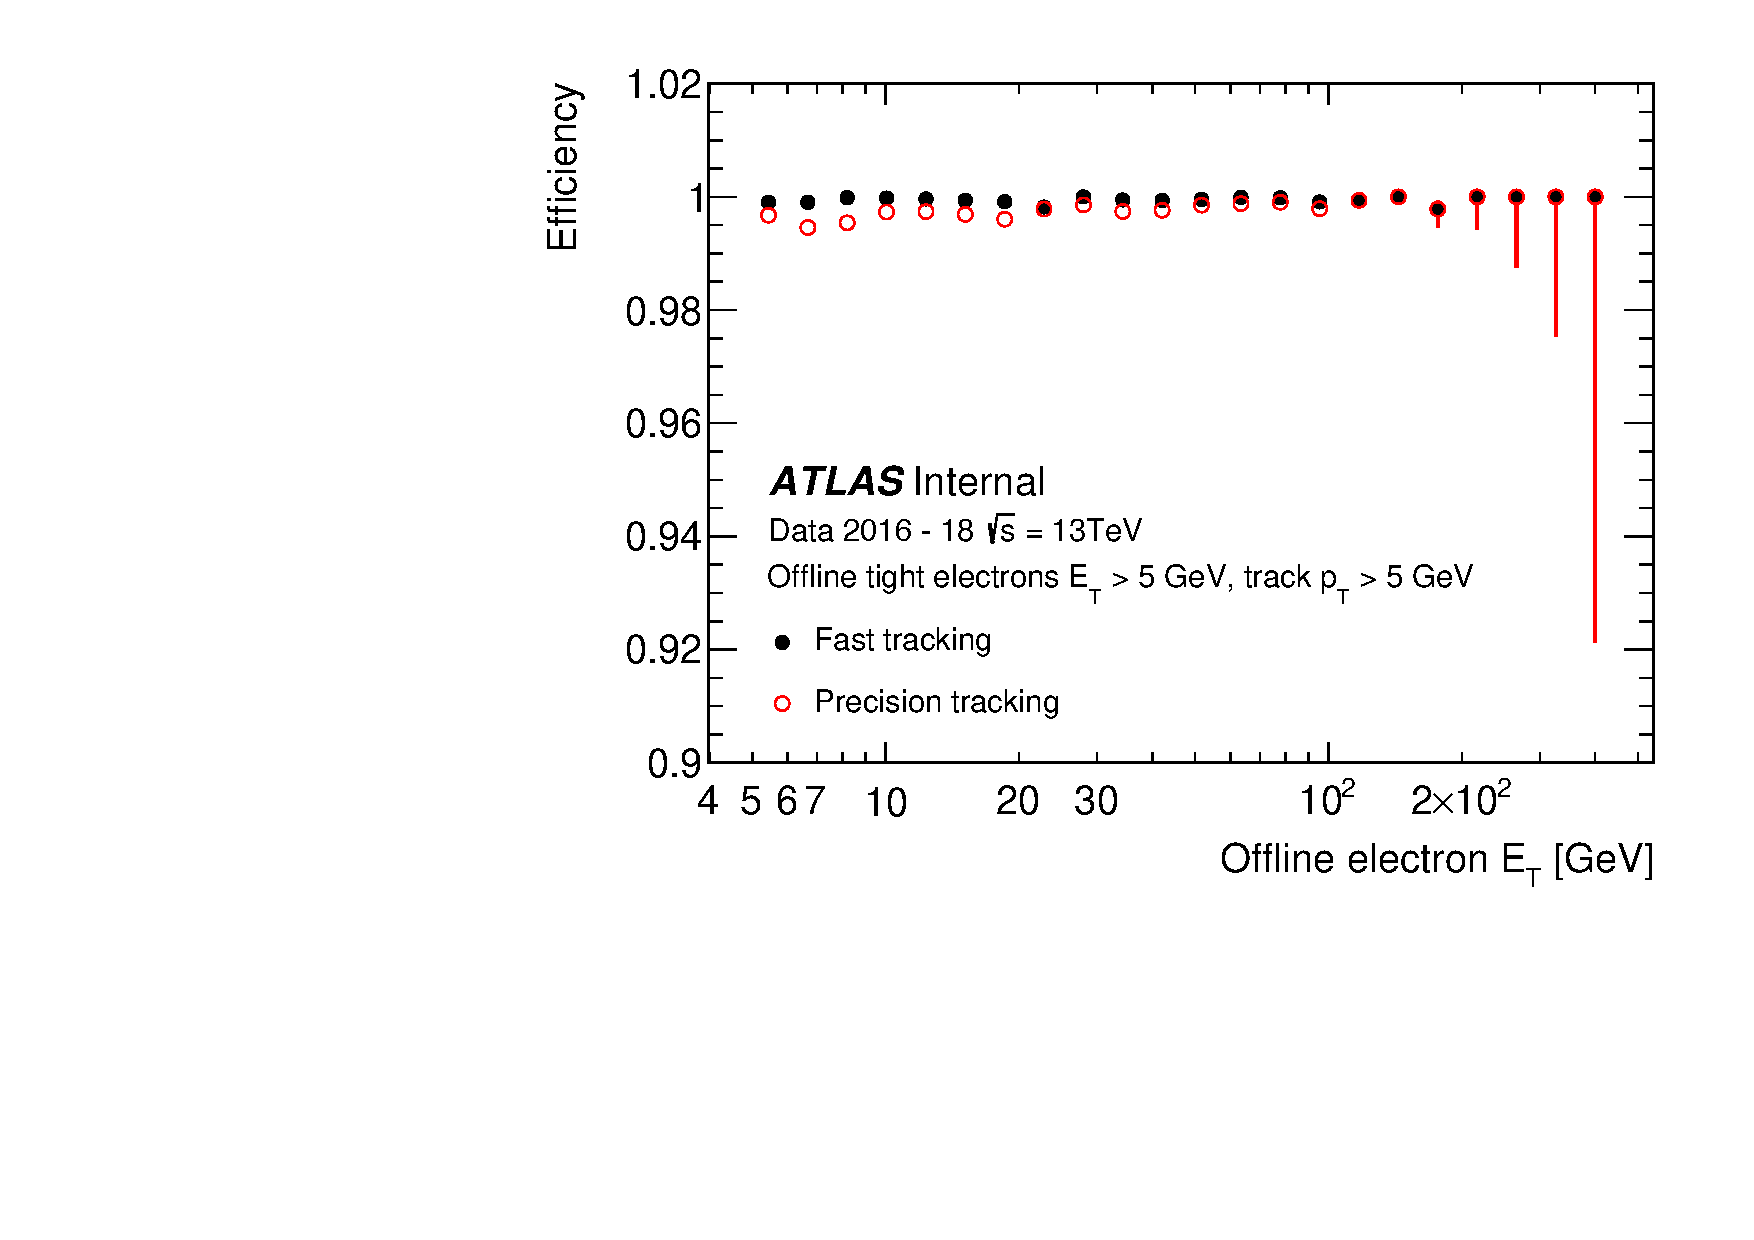
\includegraphics[width=0.45\textwidth]{IDTrig/performance/electron/HLT_eff_vs_ET}\label{fig:electron_idtrig_eff_a}}\hspace{0.05\textwidth}
			\subbottom[]{
			\includegraphics[width=0.45\textwidth]{IDTrig/performance/electron/HLT_pT_eff}\label{fig:electron_idtrig_eff_b}}\hspace{0.05\textwidth}
			\subbottom[]{
			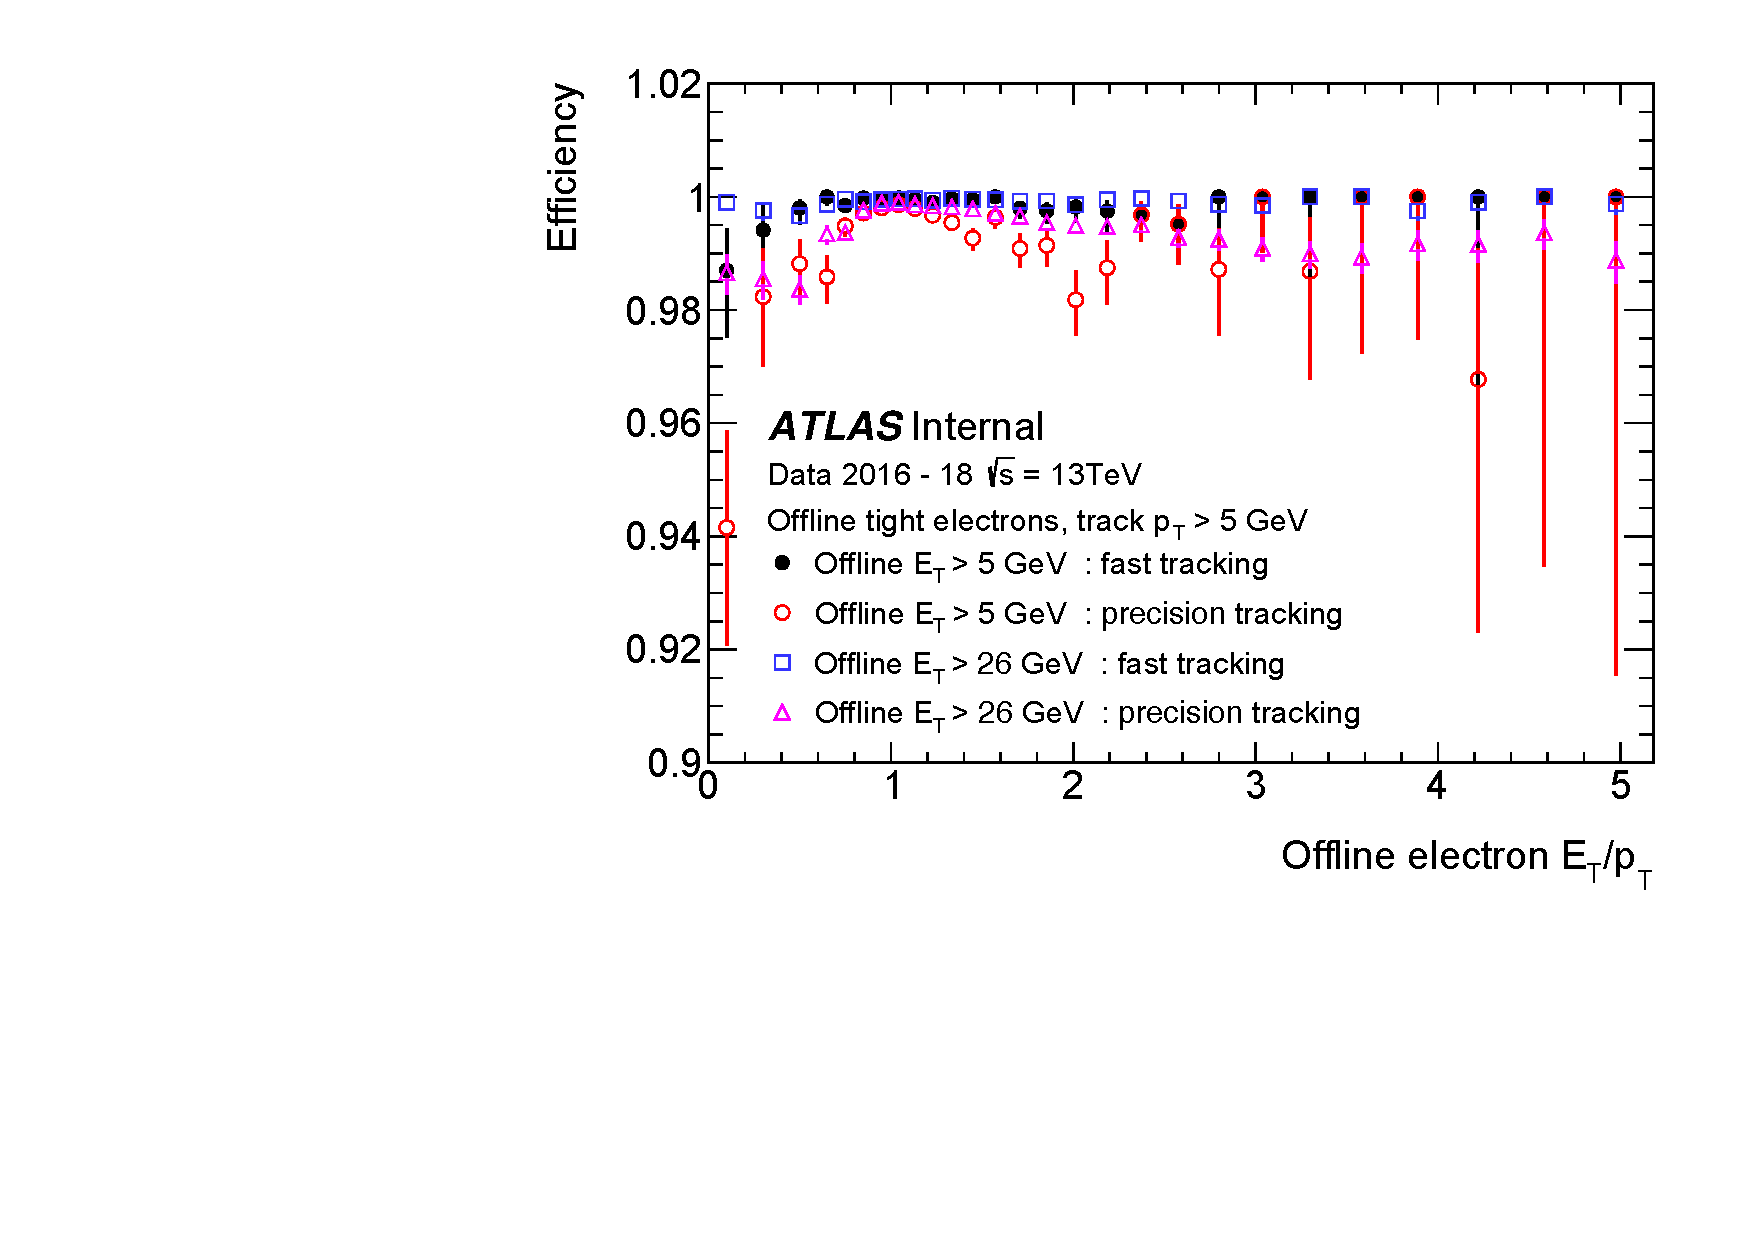
\includegraphics[width=0.45\textwidth]{IDTrig/performance/electron/HLT_eff_vs_etovptrebin26}\label{fig:electron_idtrig_eff_c}}\hspace{0.05\textwidth}
	\end{center}	
	\caption{\ac{ID} trigger efficiency as a function of (a) the offline reconstructed electron $E_T$, (b) the offline reconstructed electron track \pt, and (c) offline electron $E_T/p_T$ for electrons selected by 5 GeV and 26 GeV muon support triggers with respect to medium offline muon candidates with \pt\ $>$ 5 GeV or \pt\ $>$ 26 GeV. For the efficiency }
	\label{fig:electron_idtrig_eff}
	\end{figure}	
	Figure ~\ref{fig:electron_idtrig_eff} shows the \ac{ID} track efficiency for the 5 \gev\ and 26 \gev\ electron triggers as a function of offline electron \pt\ and $E_T$. The efficiencies for the fast and precision track finder are consistently high and exceed 99\% for all values of $E_T$. For tracks candidates from the 26 \gev\ trigger with \pt\ below 26 \gev, there is significant radiation, which may cause "kinks"  in the electron trajectory and thus decrease in the track reconstruction efficiency. Nonetheless, even for this case, the efficiency exceeds 97\%  in the low \pt\ range and reaching above 99\% at ~20 GeV.
	 For Figure ~\ref{fig:electron_idtrig_eff_c} the $E_T/p_T$ selection has been relaxed. Here, the long tail values greater than unity represent the \brem\ candidates which have radiated energy away into the calorimeter, and thus have an $E_T$ value that is greater than the track \pt. 
	 The contribution of \brem\ differs when selecting different offline $E_T$ values. For the 5 GeV trigger the \brem\ will be less then for the 26 GeV trigger. 
	Values with $E_T/p_T$ below unity represent electron candidates that have a track \pt\ that is larger than the calorimeter cluster $E_T$. This is a consequence of offline low \pt\ tracks being misreconstructed with larger values. These tracks can not have significantly more energy than the cluster, and therefore represent less reliable track \pt\ measurements. 
	There is a clear reduction in the $E_T/p_T$  efficiency for values below unity, but with only 1\% reduction for tracks where the track \pt\ is 60\% higher than might be physically possible. Tracks that have not radiated have an efficiency well over 99\%, while the efficiency for tracks that have radiated over half of their original energy is still greater than 98\%.
	
	\begin{figure}[!hbt]
	\begin{center}
		\subbottom[]{
			\includegraphics[width=0.45\textwidth]{IDTrig/performance/electron/HLT_reta_vs_eta_sigma}}\hspace{0.05\textwidth}
			\subbottom[]{
			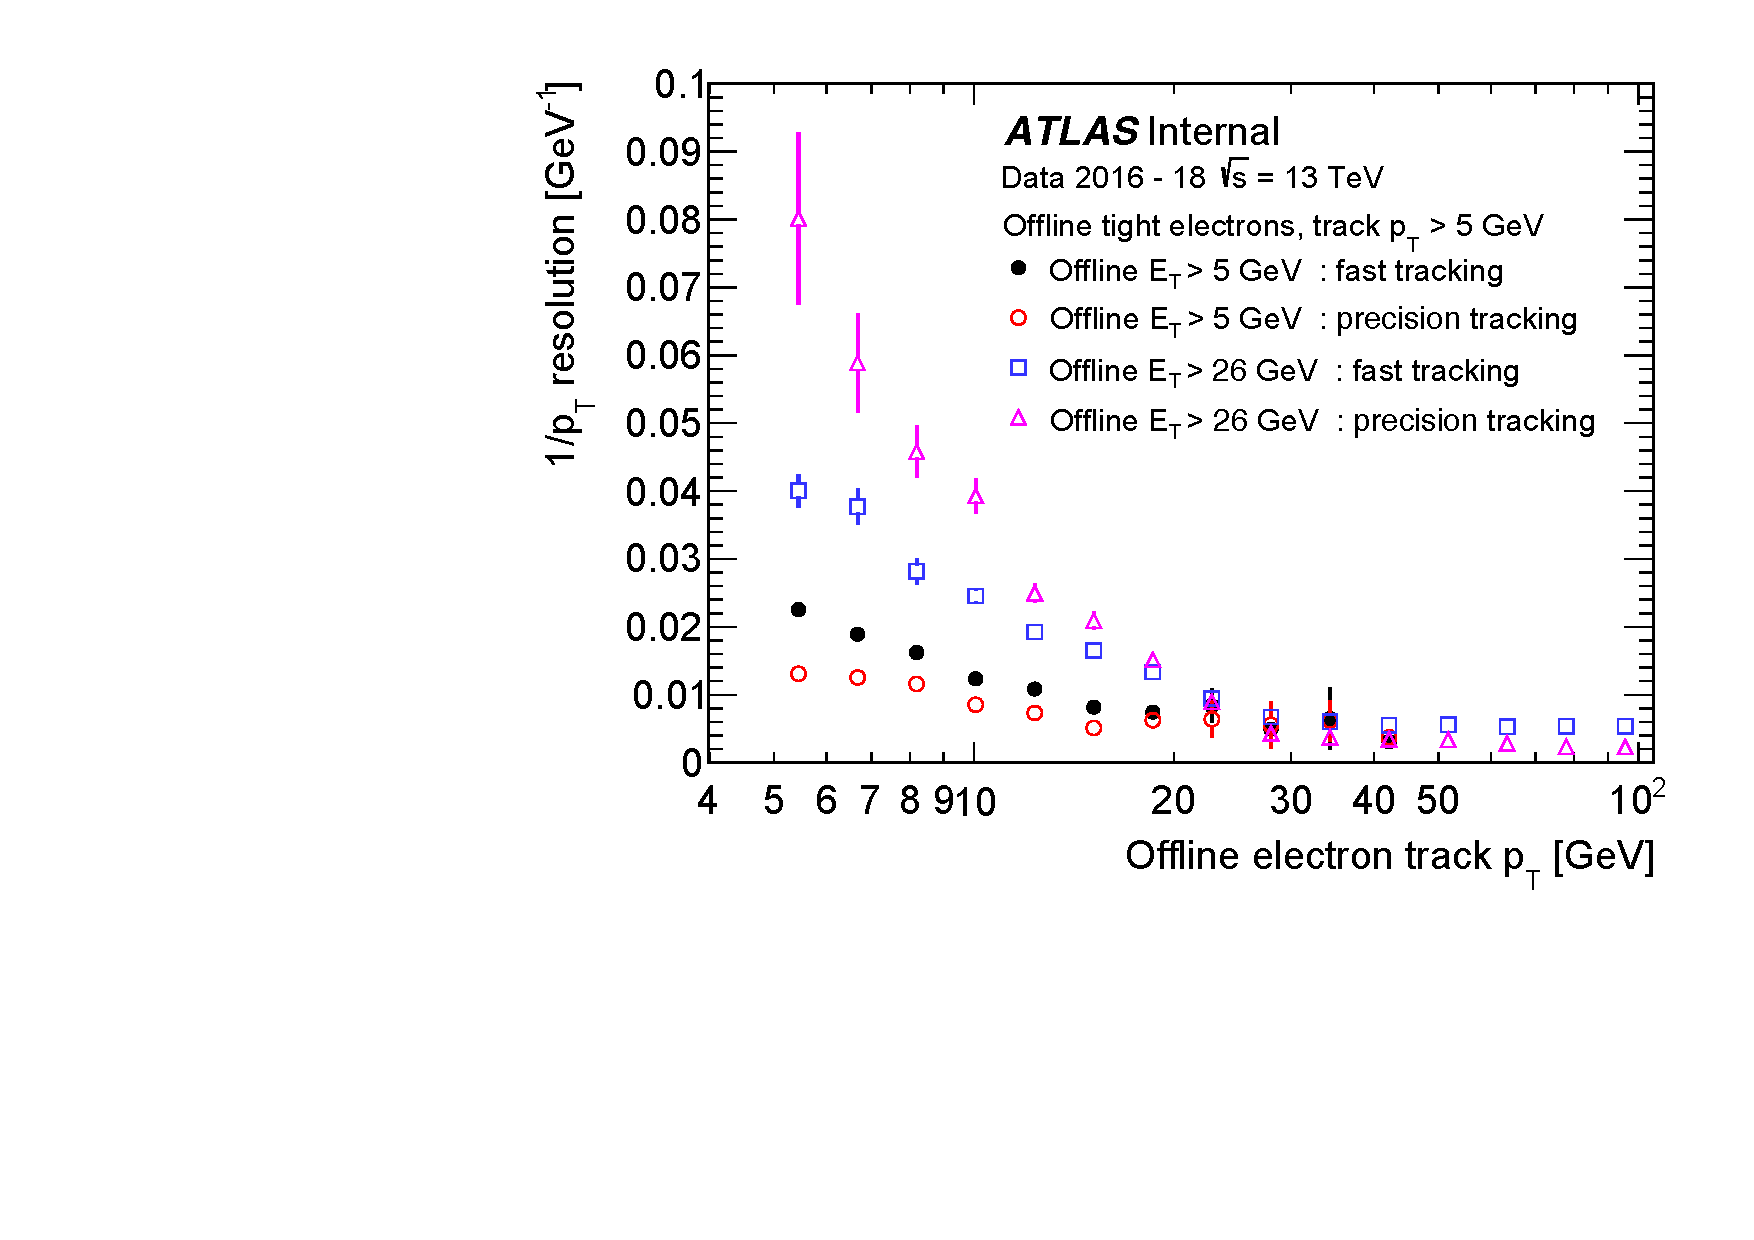
\includegraphics[width=0.45\textwidth]{IDTrig/performance/electron/HLT_ript_vs_pt_sigma}}\hspace{0.05\textwidth}
	\end{center}	
	\caption{\ac{ID} trigger track resolution for (a) track pseudorapidity ($\eta$) and (b) track 1/\pt\ as a function of offline electron $\eta$ and \pt\ for electrons selected by 5 GeV and 26 GeV electron support triggers with respect to tight offline electron candidates with \pt\ $>$ 5 GeV or \pt\ $>$ 26 GeV for both the fast and precision tracking algorithms.}
	\label{fig:electron_idtrig_res}
	\end{figure}	
	
	Figure ~\ref{fig:electron_idtrig_res} shows the resolutions for the track pseudorapidity and 1/\pt\ with respect to the $\eta$ and \pt\ of the offline track from the offline electron candidate. Unlike for the events with the 26 GeV selection, events with the 5 GeV selection have no phase space for the electron candidate near the threshold to radiate any \brem\ photons. 
	As such, tracks with \pt\ below 26 GeV from the 26 GeV trigger will correspond to electrons that have undergone a significant amount of radiation. Because of this, the resolution of these tracks will be significantly worse than for the tracks with the same \pt\ but from the 5 GeV trigger. 
	As expected, the resolutions also degrades at larger $\eta$ for both the higher and lower threshold triggers in both the fast and precision tracking. Despite the worse resolution at low \pt\ for the tracks from the 26 GeV trigger, when integrated over \pt\, the resolution is significantly better than for the lower \pt\ threshold since only a relatively small fraction of events from the 26 GeV trigger will have low \pt\ tracks. 
		\subsection*{Tau trigger}
	\noindent Figure ~\ref{fig:tau_idtrig_eff} shows the efficiency for the tau tracking with respect to the offline tracking for the offline tracks with \pt\ $>$ 1 GeV originating from decays of offline tau lepton candidates with \pt\ $>$ 25 GeV.		
		For the ID trigger tracking a multistage processes was used, as described in Section ~\ref{sec:idtrigtrack}, where the first stage runs the \ac{FTF} in a narrow \ac{RoI} in $\eta-\phi$. In this narrow $\phi$ region low-\pt\ tracks (around or below 5 GeV) may bend significantly in the solenoid magnetic field. If these tracks are on or near the edge of the \ac{RoI}, they may bend outside the region and thus are not reconstructed. 
		\begin{figure}[!htb]
	\begin{center}
		\subbottom[]{
			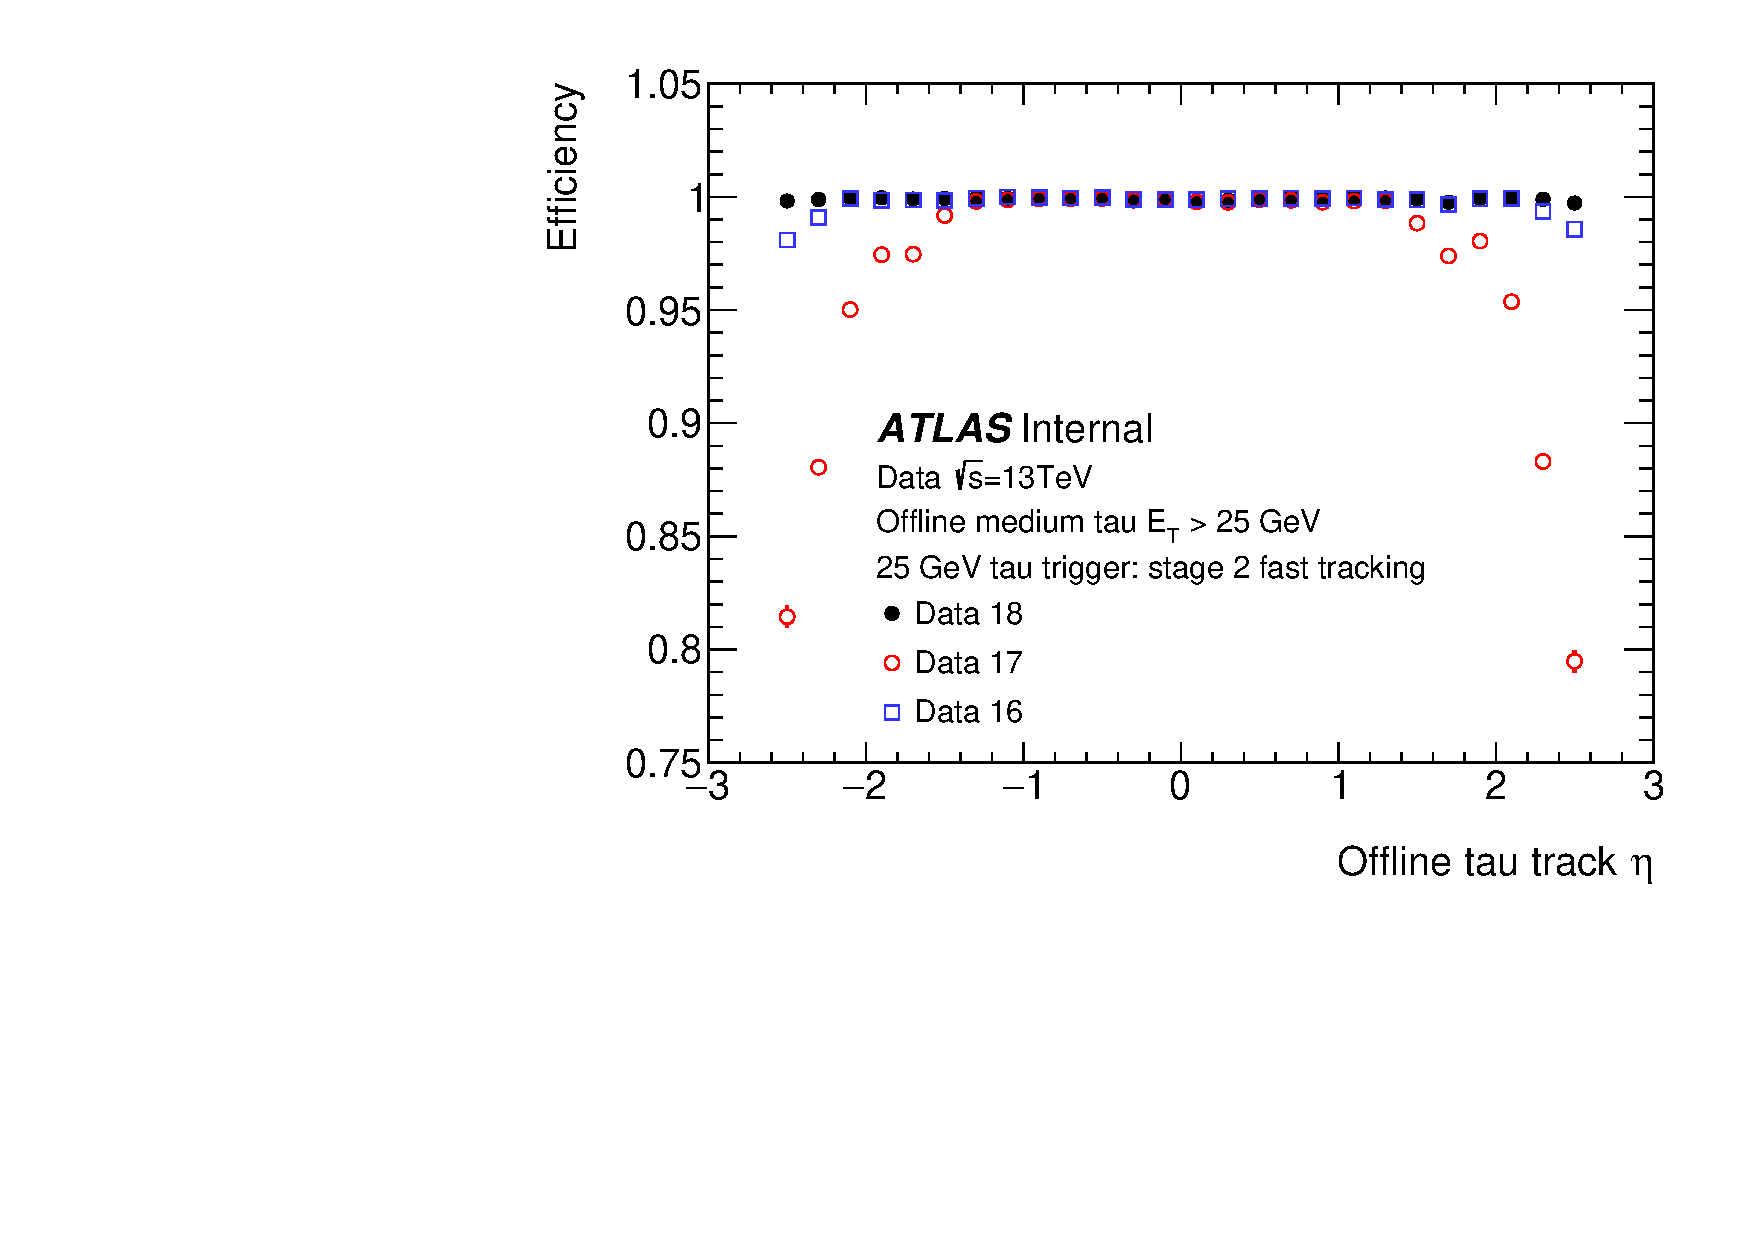
\includegraphics[width=0.45\textwidth]{IDTrig/performance/tau/HLT_eta_eff}}\hspace{0.03\textwidth}
			\subbottom[]{
			\includegraphics[width=0.45\textwidth]{IDTrig/performance/tau/HLT_pT_eff}}\hspace{0.03\textwidth}
	\end{center}	
	\caption{\ac{ID} trigger efficiency as a function of (a) the offline reconstructed tau $\eta$ comparing performance between 2016, 2017, and 2018, and (b) the offline reconstructed tau track \pt\ for the first stage fast tracking and second stage fast and precision tracking. The efficiency is evaluated for the 25 \gev\ tau performance trigger, which does not use any ID tracking information for the selection. Only tracks from tau decays with \pt $>$ 1 \gev\ are used. Bayesian uncertainties are shown.}
	\label{fig:tau_idtrig_eff}
	\end{figure}	
	
		Figure ~\ref{fig:tau_idtrig_eff}(b) shows the efficiency for the first stage fast tracking, and for the second stage fast and precision tracking from the data collected in 2018. Due to the \ac{RoI} containment issue for low \pt\ tracks  just described above, there are fewer sample of tracks near the threshold.
		This results in lower efficiencies and larger uncertainties for both the fast and precision tracking, but more significantly for the first stage fast tracking due to the narrower \ac{RoI} used in the initial stage. 
		Efficiencies are nonetheless very high, well above 96.5\% everywhere for all fast and precision tracking in first and second stage of multistage tracking and above 99\% for second stage precision tracking for tracks with \pt\ $>$ 1.2 GeV. 
		The effect of the changes to the trigger between 2016, 2017 and 2018 can be seen for the second stage fast tracking in Figure ~\ref{fig:tau_idtrig_eff}(a). In 2016 a small inefficiency was observed at large pseudorapidities because of the tightening of the second stage \ac{RoI} about the $z-$position of the leading track. 
		Approximations used in the layer positions for the seed finding were particularly affected by the worse resolution for seeds at large $\eta$, causing a significant fraction of the seeds to be rejected. The increased rate due from the higher pile-up occupancy in 2017 required some additional changes to the seed finding used for the \ac{FTF} tracking, which resulted in the further inefficiencies observed at larger $\eta$, leaving the efficiency at central $\eta$ unaffected.
		Modifications to take into account the worse seed resolution at large pseudorapidities were under development, but were not ready for the start of data taking in 2017. For 2018 the seed finding was reimplemented which restored the efficiency at large $\eta$.
		
		\begin{figure}[!hbt]
	\begin{center}
		\subbottom[]{
			\includegraphics[width=0.45\textwidth]{IDTrig/performance/tau/HLT_rd0_vs_eta_sigma}}\hspace{0.03\textwidth}
			\subbottom[]{
			\includegraphics[width=0.45\textwidth]{IDTrig/performance/tau/HLT_rd0_vs_pt_sigma}}\hspace{0.03\textwidth}
	\end{center}	
	\caption{\ac{ID} trigger track resolution for transverse impact parameter ($d_0$) as a function of offline tau track (a) pseudorapidity $\eta$ and (b) transverse momentum (\pt), respectively.}
	\label{fig:tau_idtrig_res}
	\end{figure}	
	Figure ~\ref{fig:tau_idtrig_res} shows the resolutions for $d_0$ with respect to offline track $\eta$ and \pt. 
	As expected, the precision tracking resolution is found to be generally better than the fast tracking resolution. The fast tracking resolution is found to be vert similar between the first and second stage for tracks with offline track \pt\ $>$ 5 GeV but different for \pt\ $<$ 5 GeV. This is again due to the \ac{RoI} containment requirement discussed above. When integrating over \pt, the resolution is between 15-20 $\mu$m for all pseudorapidities. 
		\subsection*{\textit{b}-jet trigger}
		The efficiency for the tracking as a function of pile-up interactions \mubar\ from both stages of the \textit{b}-jet multistage tracking process is shown in Figure ~\ref{fig:bjet_idtrig_eff}(a), while \ref{fig:bjet_idtrig_eff}(b) compares the precision and fast tracking efficiencies as a function of offline track \pt\ for the jet tracking from the 55 \gev\ and 150 \gev\ threshold triggers. For the vertex finding only tracks with \pt\ $>$ 5 \gev\ are reconstructed and thus only offline tracks with \pt\ above 5 \gev\ have been selected. For offline tracks above ~1.2 \gev\ the second stage fast tracking efficiency is better than 99.5\% for both 55 \gev\ and 150 \gev\ threshold triggers. For tracks near 1 \gev\ the fast tracking efficiency is better than 98\% but the precision tracking efficiency is approximately 85\%\footnote{This is not shown on figure as it would extend the axis range making more relevant features of the distributions more difficult to discern.}. This is a consequence of placing a 1 \gev\ cut on tracks from the precision tracking in teh \textit{b}-jet signature for processing latency reasons. The small drop in efficiency with increasing \mubar, which is more significant for the precision tracking, is driven largely by the lower efficiencies at low \pt.  
		\begin{figure}[!htb]
	\begin{center}
		\subbottom[]{
			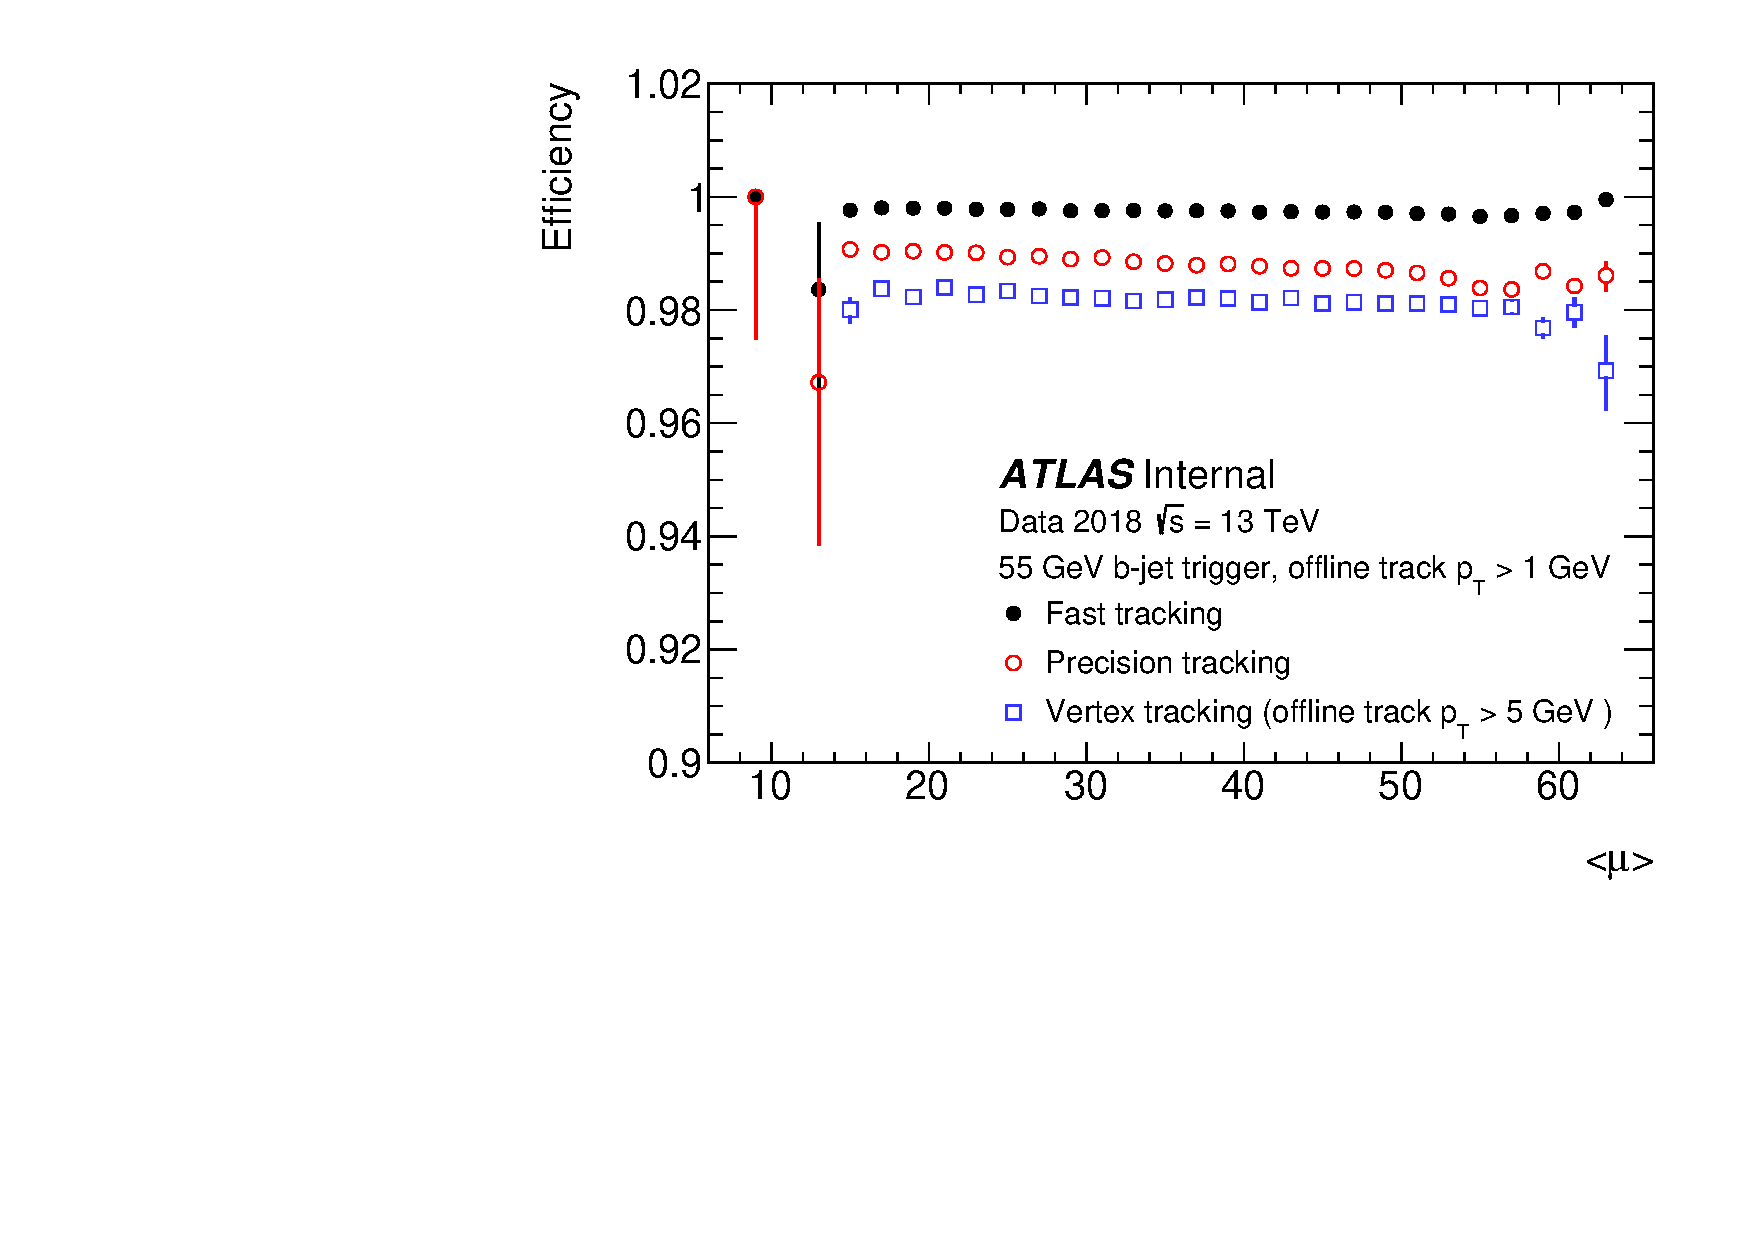
\includegraphics[width=0.45\textwidth]{IDTrig/performance/bjet/HLT_eff_vs_murebin2}}\hspace{0.03\textwidth}
			\subbottom[]{
			\includegraphics[width=0.45\textwidth]{IDTrig/performance/bjet/HLT_pT_eff}}\hspace{0.03\textwidth}
	\end{center}	
	\caption{\ac{ID} trigger efficiency as a function of (a) the mean pileup interaction multiplicity \mubar, comparing the \ac{RoI} based jet tracking with vertex tracking and (b) the offline reconstructed jet track \pt\ for the second stage fast and precision tracking, evaluated for the 55 \gev\ and 150 \gev\ \textit{b}-jet triggers. Bayesian uncertainties are shown.}
	\label{fig:bjet_idtrig_eff}
	\end{figure}	
	
	Figure ~\ref{fig:bjet_idtrig_res} shows the \ac{ID} trigger track $d_0$ resolutions as a function of $\eta$ and offline track \pt\ from the fast and precision tracking from the second stage of the \textit{b}-jet trigger for the 55 \gev\ and 150 \gev\ signatures.  As expected the precision tracking provides significantly better resolutions for the whole $\eta$ range and for $d_0$ values at lower track \pt. However, there is also a slight degradation of the $d_0$ resolution with increasing \pt\ for the high $E_T$ jet trigger. This is correlated with a slight loss of pixel pixel hits and thus corresponds to a loss in efficiency for the precision tracking at higher \pt, as found in figure ~\ref{fig:bjet_idtrig_eff}. When integrating over \pt, the resolution for the \textit{b}-jet \ac{ID} trigger second stange precision tracking is between 20-30 (20-35) $\mu$m for the 50 (150) \gev\ trigger.
	\begin{figure}[!hbt]
	\begin{center}
		\subbottom[]{
			\includegraphics[width=0.45\textwidth]{IDTrig/performance/bjet/HLT_rd0_vs_eta_sigma}}\hspace{0.03\textwidth}
			\subbottom[]{
			\includegraphics[width=0.45\textwidth]{IDTrig/performance/bjet/HLT_rd0_vs_pt_sigma}}\hspace{0.03\textwidth}
	\end{center}	
	\caption{\ac{ID} \textit{b}-jet trigger track resolution for transverse impact parameter ($d_0$) as a function of offline \textit{b}-jet track (a) pseudorapidity and (b) transverse momentum.}
	\label{fig:bjet_idtrig_res}
	\end{figure}	
	
		\subsection*{Vertex Finding}
		%The more robust but less accurate histogramming vertex algorithm is used for the online vertex selection to identify vertex candidates for those events where the offline based vertex algorithm failed to find a vertex. 
		For the measurement of performance, the online vertex efficiency is calculated for the single offline vertex candidate from the bunch crossings with the highest sum of the squared transverse momenta. 
		Figure ~\ref{fig:vertex_idtrig_eff} shows the efficiency for identifying the vertex candidates in the trigger for the 110 \gev\ and 420 \gev\ triggers, as a function of the offline track multiplicity in the super \ac{RoI} and the mean pile-up interaction multiplicity of the event.
\begin{figure}[!htb]
	\begin{center}
		\subbottom[]{
			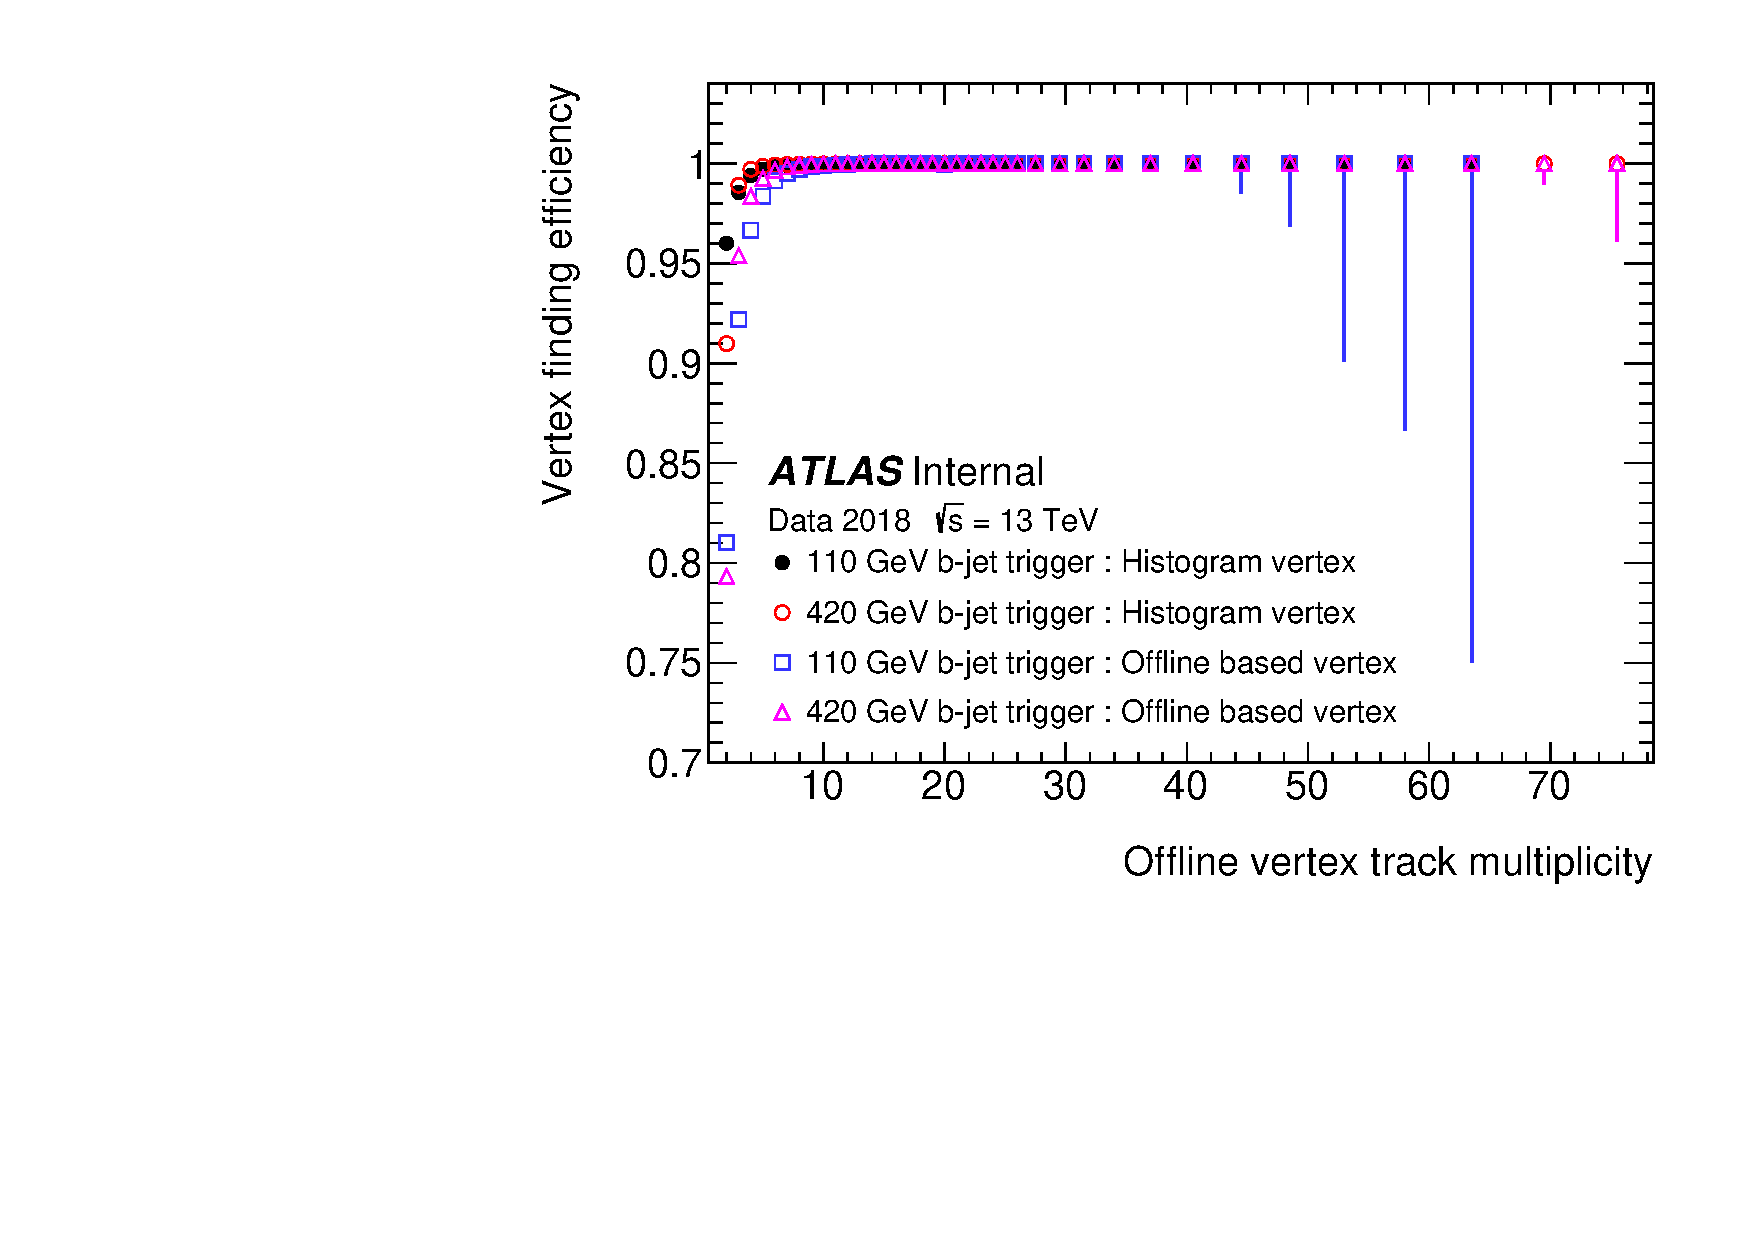
\includegraphics[width=0.45\textwidth]{IDTrig/performance/vertex/HLT_ntrax_eff}}\hspace{0.03\textwidth}
			\subbottom[]{
			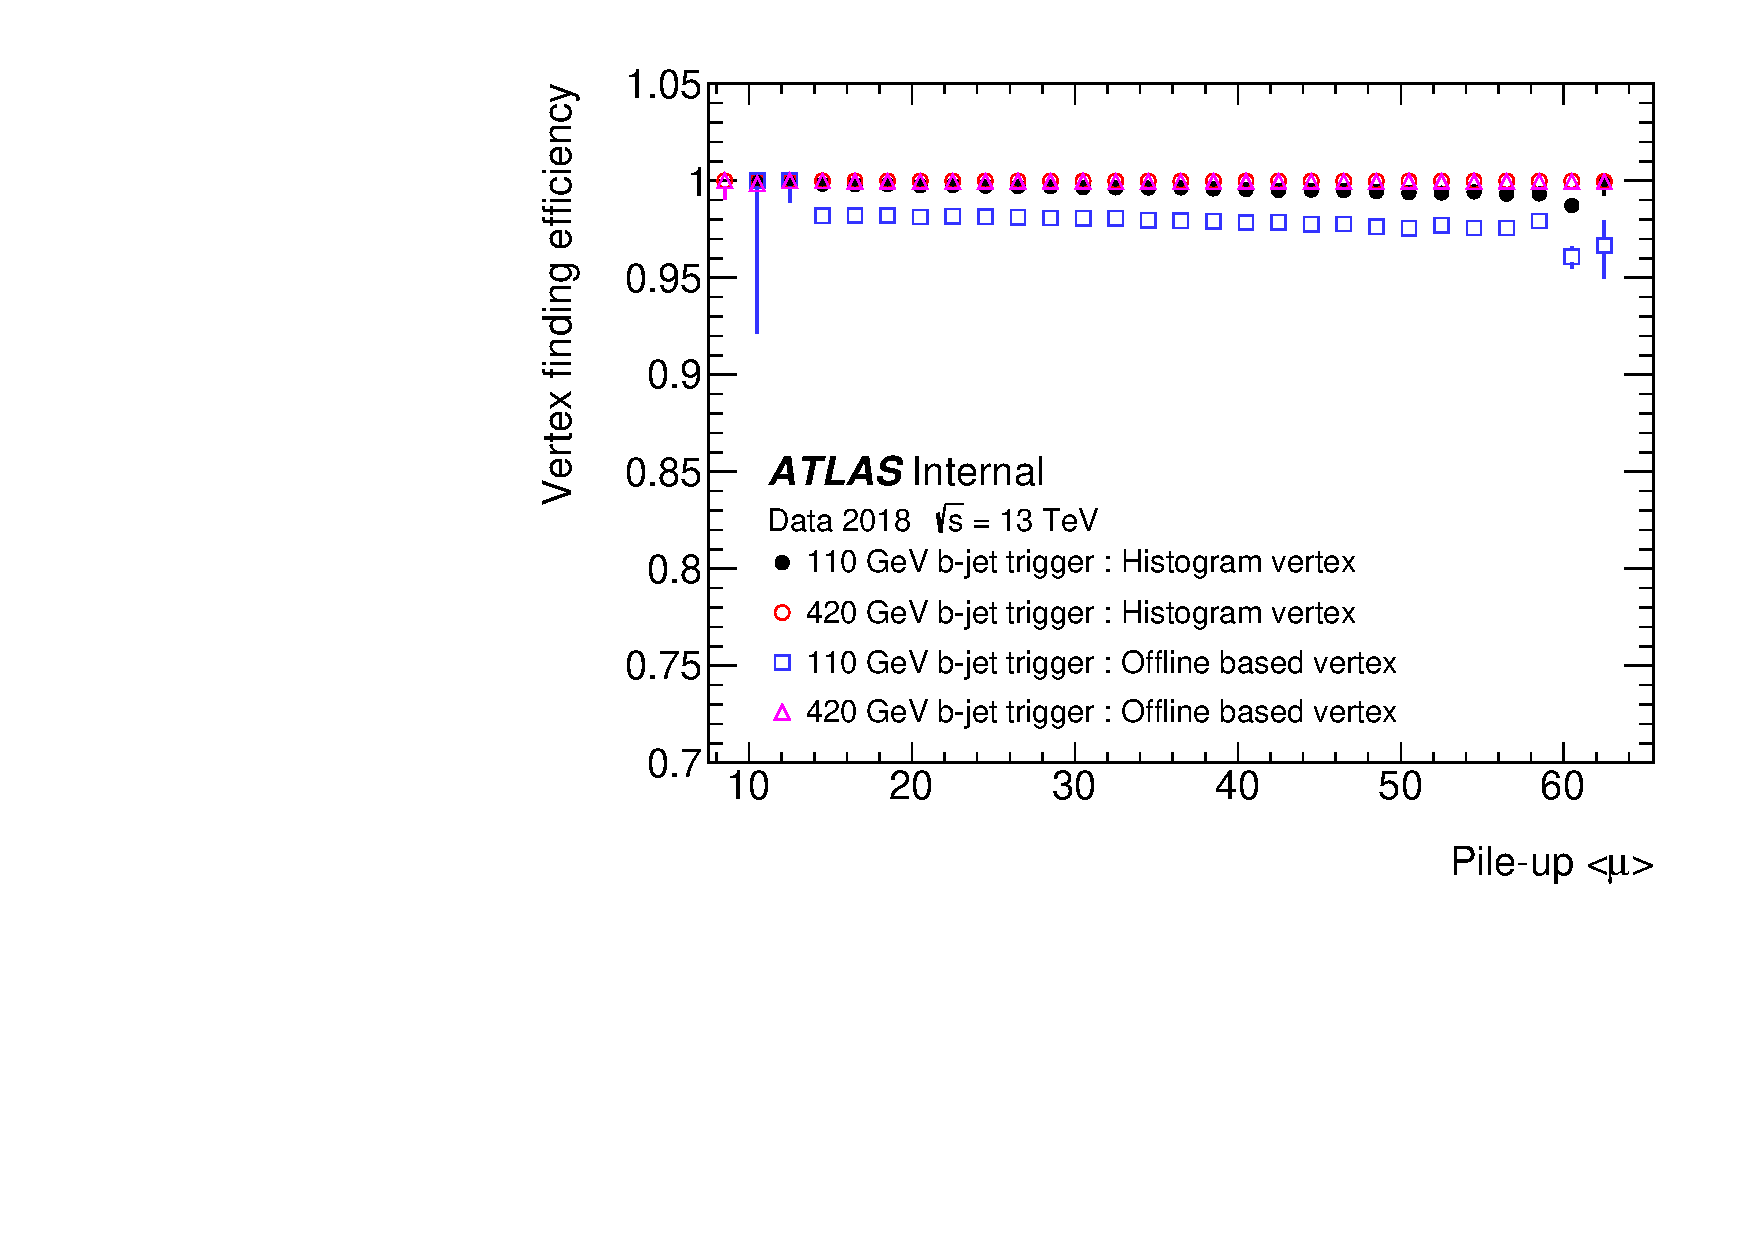
\includegraphics[width=0.45\textwidth]{IDTrig/performance/vertex/HLT_mu_eff}}\hspace{0.03\textwidth}
	\end{center}	
	\caption{The vertex algorithm \ac{ID} trigger efficiencies for 110 \gev\ and 420 \gev\ $E_T$ threshold \textit{b}-jet triggers. The efficiencies versus (a) the offline track multiplicity for tracks in the super \ac{RoI}, and (b) the mean pile-up interaction multiplicity are shown. Bayesian uncertainties are shown.}
	\label{fig:vertex_idtrig_eff}
	\end{figure}	
		
	A steep rising edge is found for the vertex finding algorithms with increasing offline track multiplicity. For the histogram based algorithm full efficiency is reached for event with more than four vertex tracks within the \ac{RoI}, while for the offline based algorithm full efficiency is reached only for events with more than eight 	vertex tracks.
	This is due to the tighter track quality required by the offline based algorithm. Due to this higher track quality requirement, some vertices with only a few tracks in the super \ac{RoI} may not have any tracks remaining with which to form a vertex once the tracks with lower quality are removed. 
	Higher $E_T$ jet triggers will have significantly higher tracks multiplicities and larger average tracks \pt\, making the probability of the track multiplicity for a pile-up vertex matching or exceeding that for the interaction of interest significantly lower. Both algorithms show a reduction in the efficiency as \mubar\ increases. This is due to the increased possibility of for offline selection to misidentify the jet vertex candidate within the super \ac{RoI}. Therefore, as the pile-up interaction multiplicity increases within an event, so do the chances of there being additional tracks from additional vertices within the super \ac{RoI}.
	 The lower overall efficiency of the offline based algorithm, particularly for the lower $E_T$ threshold trigger, is due to the lower overall track multiplicity in the events passing the trigger. The trigger is therefore still on the rising edge of the efficiency distribution for many events, causing a lower overall efficiency as a function of \mubar. For the higher $E_T$ thresholds triggers, the multiplicity is higher and thus the algorithm is further along the efficiency curve for most events, resulting in a higher overall efficiency. 
		\begin{figure}[!hbt]
	\begin{center}
		\subbottom[]{
			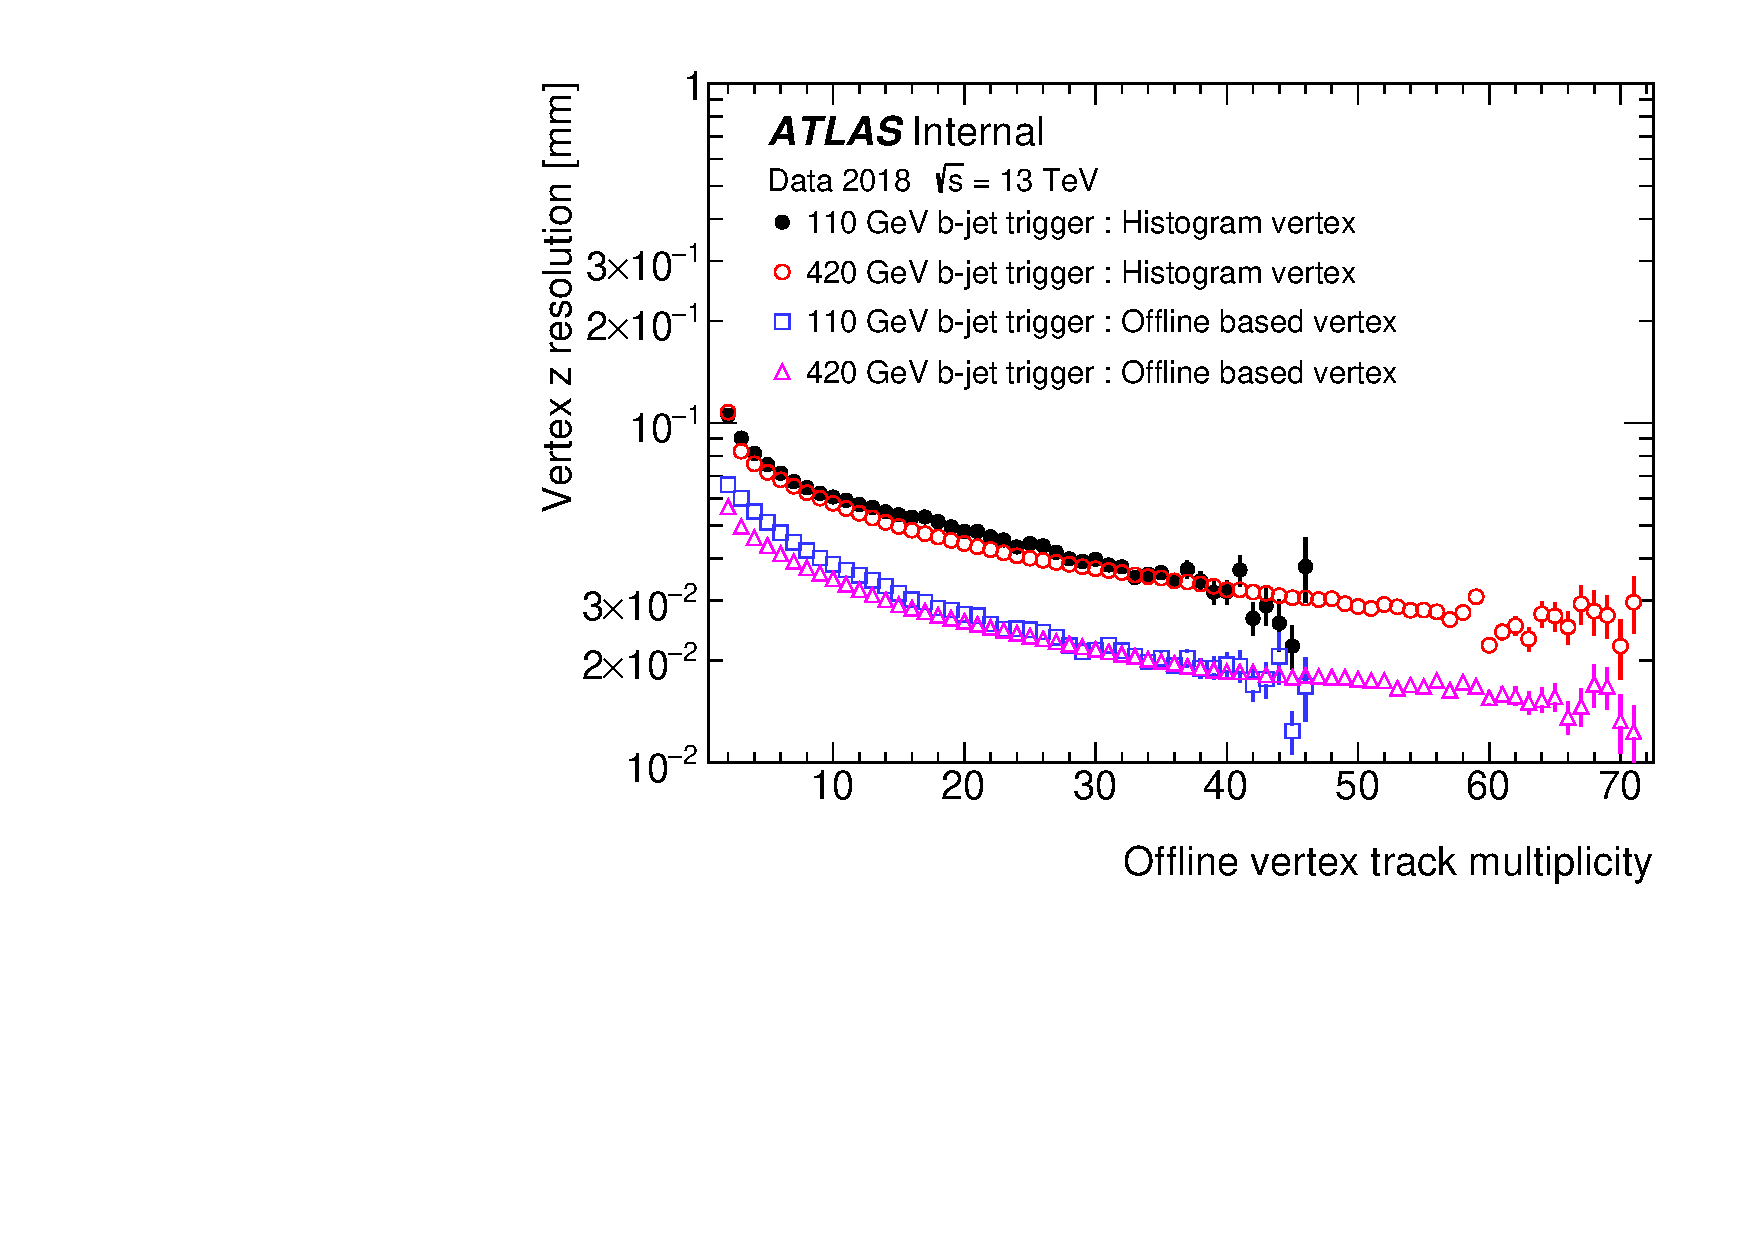
\includegraphics[width=0.45\textwidth]{IDTrig/performance/vertex/HLT_rdz_vs_ntrax_sigma}}\hspace{0.03\textwidth}
			\subbottom[]{
			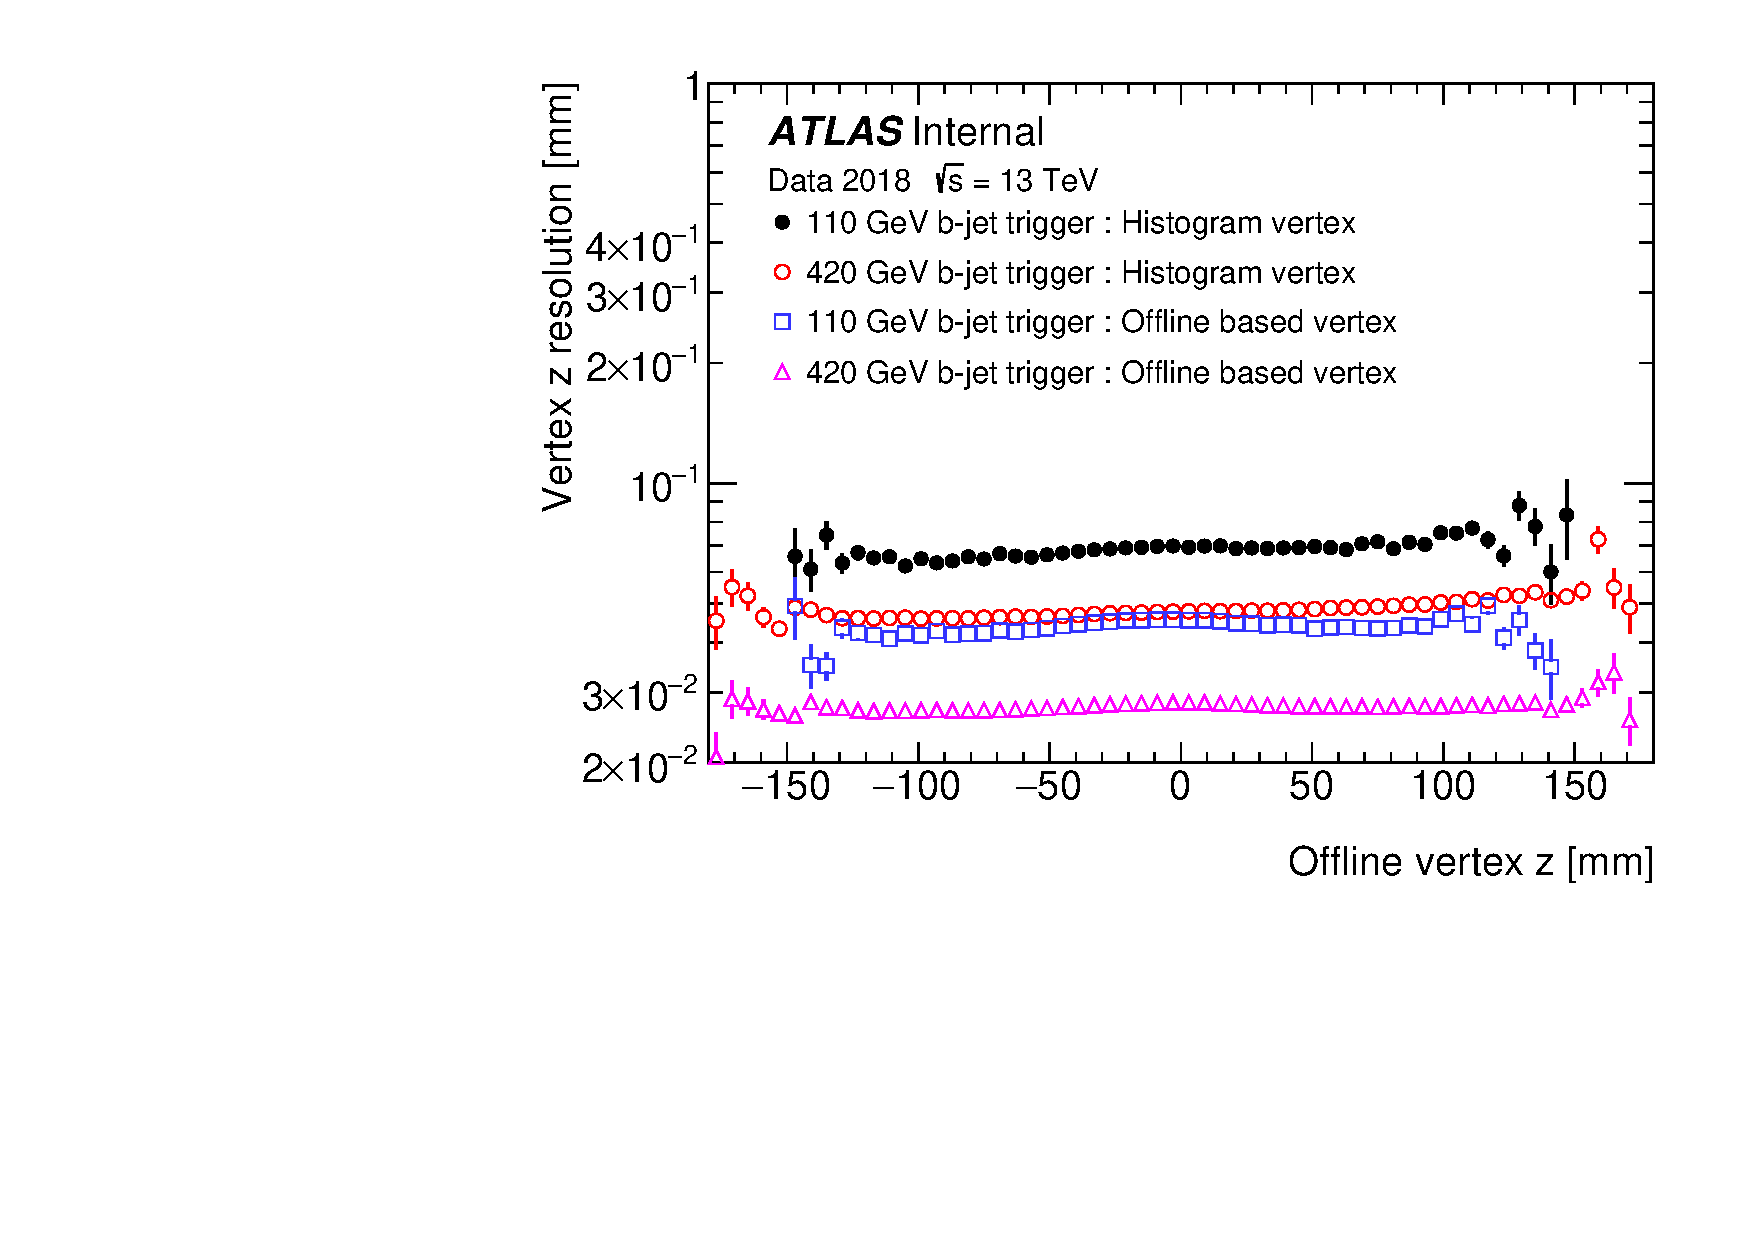
\includegraphics[width=0.45\textwidth]{IDTrig/performance/vertex/HLT_rdz_vs_zed_sigma}}\hspace{0.03\textwidth}
	\end{center}	
	\caption{\ac{ID} vertex reconstruction vertex  $z$  position track resolution for 110 \gev\ and 420 \gev\ \textit{b}-jet triggers as a function of (a) the offline track multiplicity and (b) the offline $z$ vertex position.}
	\label{fig:vertex_idtrig_res}
	\end{figure}		

	The resolution of the vertex $z$ for both online algorithms as a function of the offline track multiplicity and the offline  $z$  vertex positions is shown in Figure ~\ref{fig:vertex_idtrig_res}.
	The resolution on the vertex  $z$  position for both online algorithms improves with increasing track multiplicity, with the offline based algorithm showing a significantly better resolution. The resolution of both algorithms improves logarithmically with increasing track multiplicity from 100 $\mu$m and 70 $\mu$m at low track multiplicity, to 30 $\mu$m and 20 $\mu$m at 50 tracks, for the histogram and offline based algorithms respectively. The higher resolution observed for the high $E_T$ threshold trigger is due to the larger average \pt\ of tracks from the higher $E_T$ jet triggers, such that the track  $z$  positions themselves have an intrinsically better  $z$  resolution.
	The resolution as a function of vertex  $z$  position is largely constant with a small degradation at around  $z$  mm, and a slight trend towards better resolutions for more negative  $z$  for the lower $E_T$ threshold triggers. This is especially evident for the histogram based algorithm.
	
	
	\section{Summary}
	This chapter presented the \ac{ATLAS} trigger with particular interest in the \ac{ID} trigger and tracking algorithms and corresponding performance. 
	The performance in terms of efficiency with respect to the offline algorithms, and resolutions of the \ac{ID} tracking algorithms for the main physics signatures needed by the \ac{ATLAS} physics program: muon, electron, tau, and b-jet, are shown. 
	The performance has been excellent event at the very high interaction multiplicities observed at the end of data taking in 2018. The results have been submitted for publication to \color{red} ADD JOURNAL ONCE PUBLISHED \color{black} and have been presented by the author at many conferences, including at: the Large Hadron Collider Physics conference in 2018, The Institute of Electrical and Electronics Engineers Realtime Conference in 2018, and the International Conference on High Energy Physics in 2020.
	The study of the performance of these triggers has been part of the \textit{qualification task}\footnote{To become an \ac{ATLAS} author active \ac{ATLAS} researchers must spend 50\% of their time on a technical task (for the first year) and 30\% the following year.}
	of the author.
	The excellent performance of the \ac{ID} trigger algorithms demonstrates how the \ac{ID} trigger continues to lie at the heart of the trigger performance and plays an essential r$\mathrm{\hat{o}}$le in the \ac{ATLAS} physics programme.